%\section{section} (h2)
%\subsection{subsection} (h3)
%\subsubsection{subsubsection} (h4)
%\paragraph{paragraph} (h5)
%\subparagraph{subparagraph}

\textit{Ice-Bound}'s system is a custom combinatorial narrative engine co-created with Aaron Reed, culminating in the release of an indie game in 2014. It's a good case study of an exploratory generative narrative system taken all the way from theoretical implementation to exemplary media experience. \textit{Ice-Bound} won the award for Best Story / World at IndieCade 2014, in addition to being featured in the Independent Games Festival and SXSW.

%%signposting%%
We'll start with detailing the specific experience we were trying to create: an interactive narrative where players can sculpt the story to explore it, through the use of combinatorics. Then, some related systems and works in the area of combinatorial narrative will be explored in Section \ref{sec:ib-related-works}. Thus contextualized, we'll then do a deep dive into \textit{Ice-Bound}'s system specifics in Section \ref{subsec:ice-bound-summary}. This will lead to our application of the Authorial Leverage Framework. First, we will profile the Traversability challenge of the work (driven by the combinatorics and large state space) in Section \ref{subsec:icebound-traversability}. Then in Section \ref{subsec:icebound-authorability} we'll show how that challenge was answered, in this case primarily through focusing on authorial Clarity and increasing that through authoring tools.
%%signposting%%

\section{Experience Challenge}\label{sec:ib-experience-challenge}

\textit{Ice-Bound} conceptually started as a pitched project for the ``Envisioning the Future of the Book" grant from the Center for Book and Paper Arts at Columbia College Chicago. This grant was looking for works that could ``take both virtual and physical manifestations, examining the advantages of each and how the interplay between the two can be leveraged to provide a comprehensive and powerful expression" \cite{rhizome_2012}. Specifically, they were looking for physical artists' books that would exist in dialogue with a digital system.

We took the prompt of what the ``future of books" would be, and extrapolated it out (somewhat facetiously) to ``what use are physical books in a future where all books are digital?" The seed that would grow to be our core story came from a sardonic answer: DRM (digital rights management).

For \textit{Ice-Bound}, there are two components. A physical printed book, \textit{The Ice-Bound Compendium}, and the digital game: \textit{The Ice-Bound Concordance}. The frame narrative of the work positions it in the future, where the primary reason for printed books' existence is that human-level AIs cannot easily access their information. The \textit{Compendium}, therefore, is a collection of secret materials and ``transmissions" about the main character of the work, Kris Homquist (or as his AI simulacrum is known: KRIS). It was put in print form to prevent him from being able to access it, as a simulacrum can easily access all digital information, but can be easily prevented from accessing the physical world.

The character you interact with, KRIS, is an AI created from a brain scan of Kris Holmquist, a popular writer. Kris died before he could finish his masterpiece \textit{Ice-Bound}, and because he was under contract with a publisher for it, they decided to ``spin up" a copy of him to finish it. Unfortunately, the personal issues that hounded Kris make it impossible for KRIS to finish the work, or decide what is the best way for the story to go (in a very ``life imitates art" manner). The player, in this case, is ``assigned" to KRIS to help shepherd him through the editing process, deciding which of the many ways the story can go is the ``correct one", and in the course of that, forcing him to confront the past mistakes and issues of his life that kept him from finishing his magnum opus.

That is a very linear and simplified version of the story, of course. The book material is meant to interface with the digital game in a collage-like and orderless manner--there is no correct order to read the \textit{Compendium} in, and no guarantee that a certain section of the story will be seen before another. It is meant to be taken in as a sort of ``narrative possibility space" whose details are teased out by determining where the voices are in chorus, not in discord.

While we did not receive that particular grant, we came away from it with a solid project proposal. When another grant--UCSC's SPIN (Student Project INcubator) Studio grant--became available, we used that application process to expand upon the proposal with a digital prototype.

%%%%%%%% BEGIN FIGURE %%%%%%%%%%%%%%%%%%%%%%%%%%%%%%%%%

\begin{figure}
    \centering
    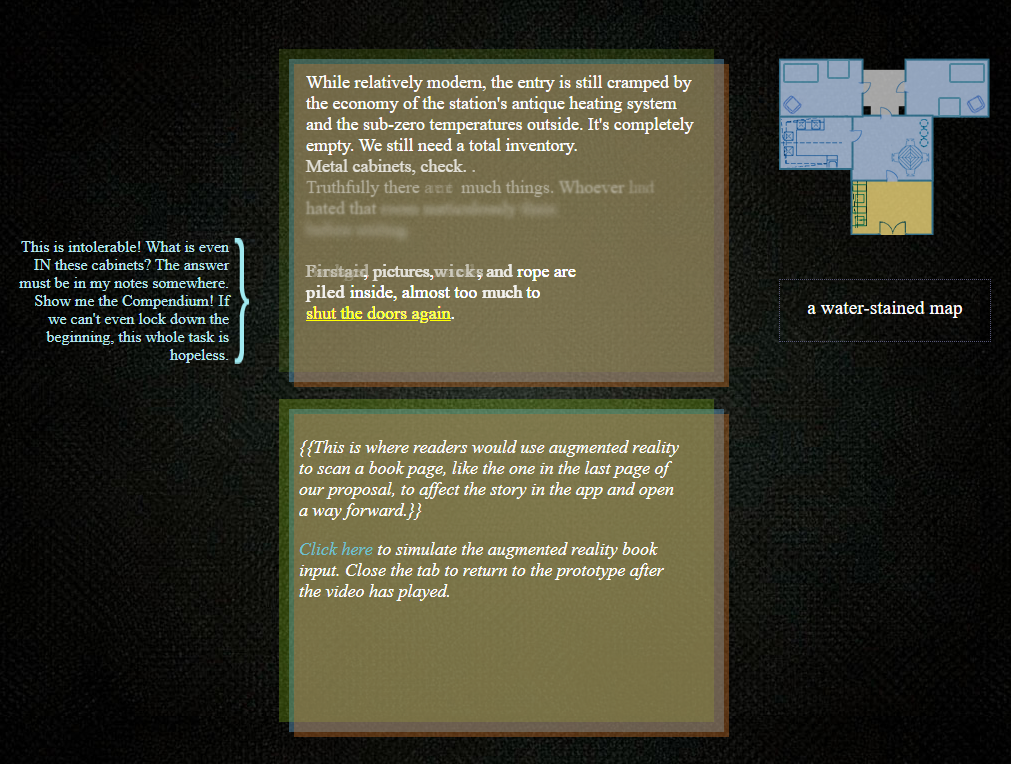
\includegraphics[width=\textwidth]{figures/2-Ice-Bound/digital-prototype.png}
    \caption{Early, non-combinatorial prototype of \textit{Ice-Bound}.}
    \label{fig:digital-prototype}
\end{figure}

%%%%%%%%%%%% END FIGURE %%%%%%%%%%%%%%%%%%%%%%%%%%%%%%%%

The initial prototype was much closer to a visual interface for a traditional text game as its central metaphor (Figure \ref{fig:digital-prototype}). We thought we would create a game in which players moved through rooms, casting ``light" on them as they moved, which would allow them to interact with the different objects within. Moving the objects to different rooms would unlock different capabilities, and change the story told on that level. This was much closer to a ``lock and key" system than a combinatoric one, although the potential for different objects in each room was the seed of the combinatorics we'd later embrace.

We still had unresolved questions about what such a design would require authoring-wise, but we knew that undertaking a dynamic narrative project could easily result in untenable authorial burden if we weren't conscious of our content creation commitments at all times of the design process.

Initially, we flirted with the idea of using Skald---Tearse's reconstruction of Turner's Minstrel system \cite{tearse_skald}---to generate narratives. Aaron Reed, the project's co-creator, had done some work with the system and had a good working understanding of it. But we dropped that early on in order to create a more bespoke system that would speak to the particular strengths targeted for our project, and whose capabilities could evolve as the design itself evolved.
%%GDoc comments%%
Before we began in earnest on the digital system design, we went through a period of paper prototyping to shed light on the types of dynamics that would emerge from the kind of interactions we wanted to foster for our target experience. This practice is well known in HCI (Human Computer Interaction) circles colloquially as the ``Wizard of Oz" technique or Oz technique, which has been around since 1975 where it was first known as the ``experimenter in the loop technique" \cite{wizard_of_oz}. Some of its first uses were in iterative prototypes of natural-language interfaces, where the experimenter would manually type out dictation spoken by the subject. As development continued, the ``wizard" became less necessary, until ultimately the program could run without intervention \cite{kelley1984iterative}. Since then, it has been used as a useful way to quickly iterate on graphical interfaces \cite{snyder2003paper} and game mechanics \cite{mayra2004player} as well as generative narrative systems \cite{cozy_mystery}.
%%GDoc comments%%
Once we began paper prototyping, it became quickly apparent that in order to control authoring burden, we would need a way to flexibly limit or group story components to reduce combinatorics where necessary. We found we could successfully gauge this by using small cards with sections of story on them, then having one person be ``the player" and ``activate" different parts of the story, while the other person played ``the computer", and used different types of rules to determine what to display to the player.

%%%%%%%% BEGIN FIGURE %%%%%%%%%%%%%%%%%%%%%%%%%%%%%%%%%

\begin{figure}
    \centering
    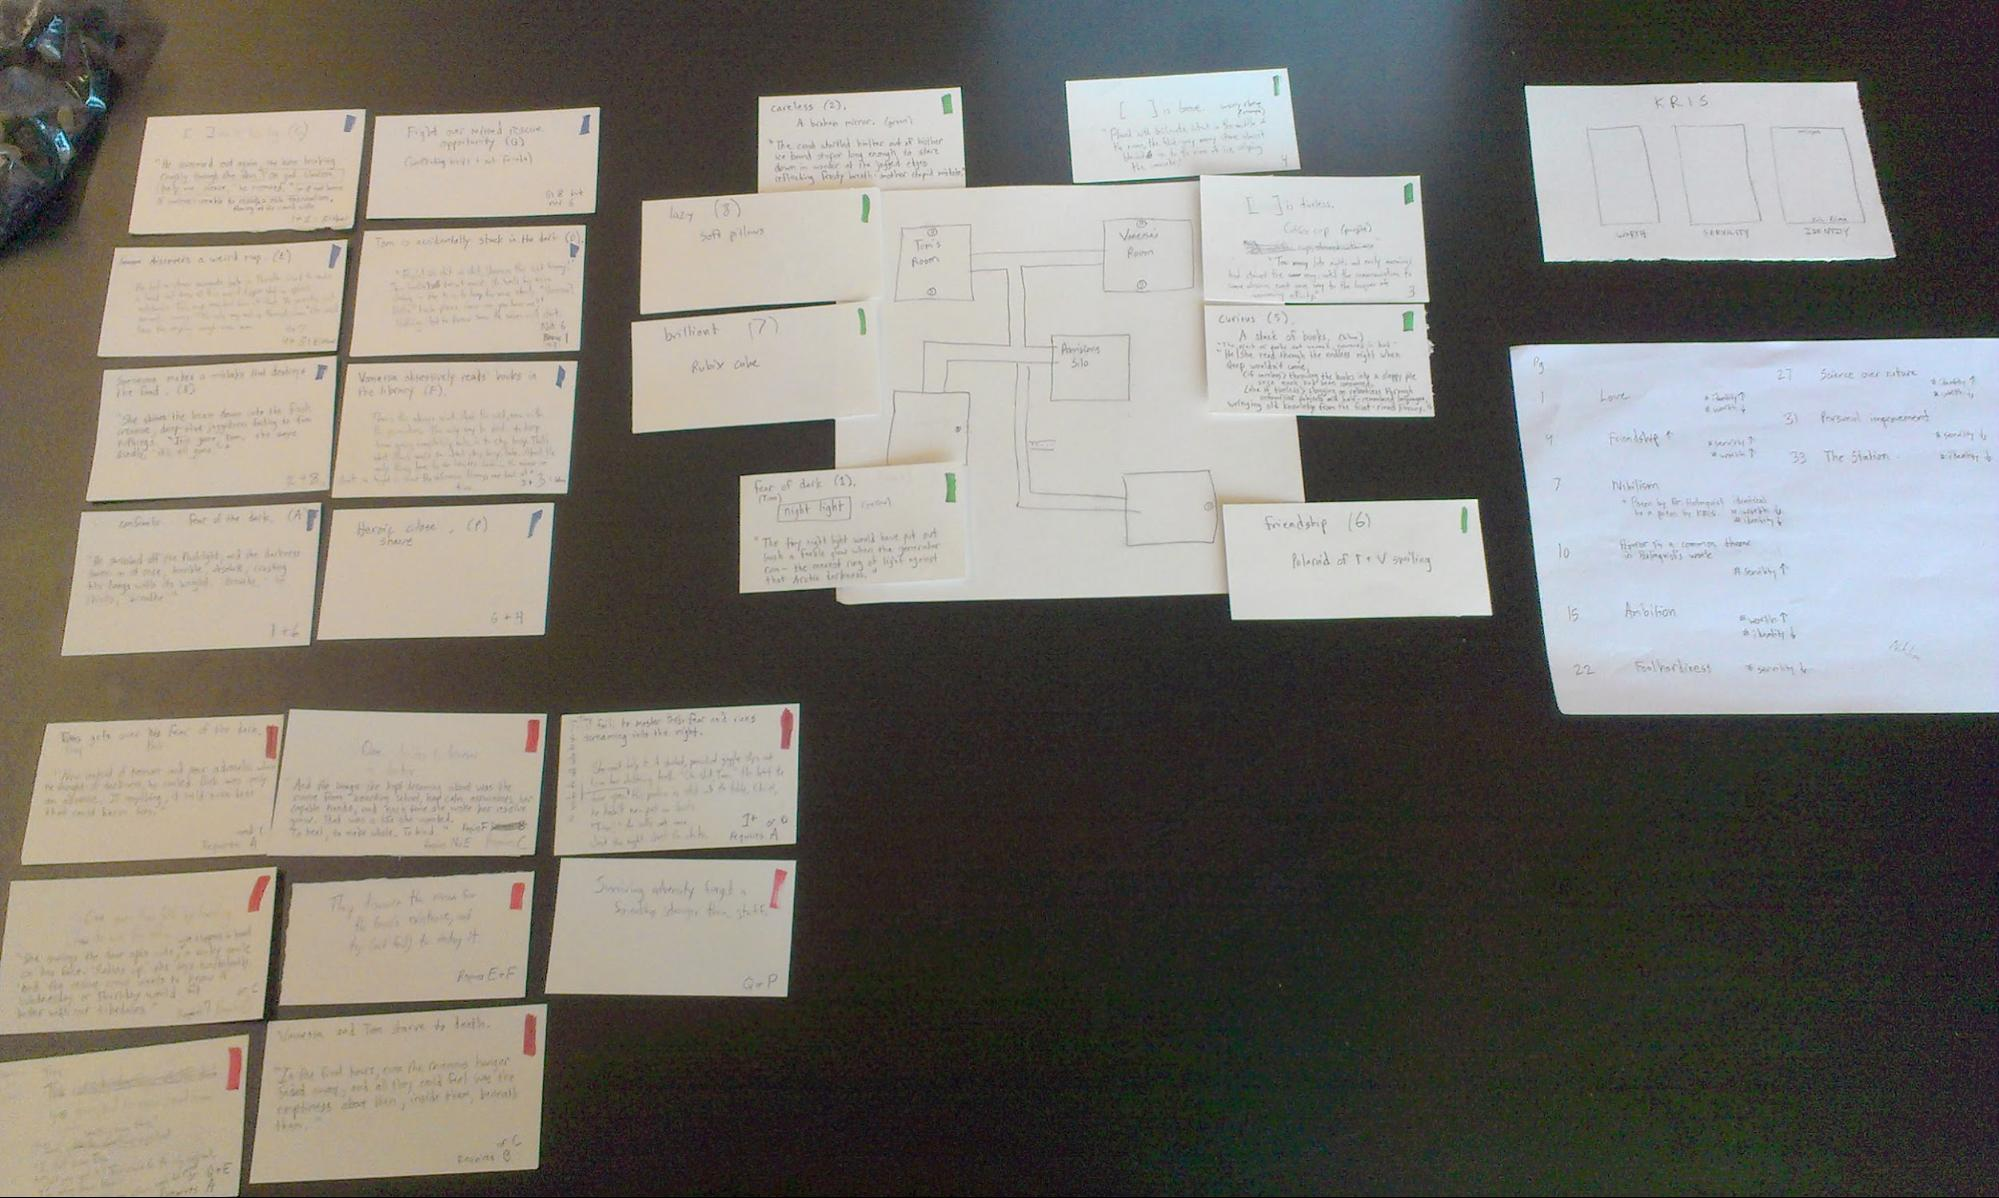
\includegraphics[width=\textwidth]{figures/2-Ice-Bound/prototype.jpg}
    \caption{Early paper prototype of \textit{Ice-Bound}, showing symbol, event, and ending cards, along with a map. The ``player" would choose symbol cards to flip over on the map, and the ``computer" would then consult the deck of events and endings, and flip over the corresponding ones.}
    \label{fig:prototype}
\end{figure}

%%%%%%%%%%%% END FIGURE %%%%%%%%%%%%%%%%%%%%%%%%%%%%%%%%

From there, we would loosen or constrain the pre-conditions on cards, coming up with new categories of pre-conditions when necessary, while also keeping an eye on how many cards we were setting ourselves up to write to fulfill all the combinations. This design process of refining the system, then refining the type of experience to provide to lean into those strengths, then refining the system further to support aspects we discovered we really needed, was very productive.

After this exploratory period of paper prototyping and iterating, we determined the two pillars of our experience were high quality hand-authored text that one would normally see in static branching narratives, but with a kind of responsiveness and granularity that would encourage exploration and playfulness with the materials of the story.

Aaron Reed detailed this best in his post-mortem \cite{reed2014ice}:

\begin{quote}
We wanted to find a core mechanic that gave us the best of both approaches: the focused, quality surface text offered by branching paths, with the sense of playful exploration allowed by simulationist works [...] one author proposed the notion of "sculptural fiction" to identify works that involve frequent small but reversible decisions, to create a play aesthetic closer to a sculptor constantly refining a work than a rat navigating a maze. The focus should be on continuous, small, reversible choices, creating a playful and exploratory feel.
\end{quote}

This, combined with longer form, static materials in the \textit{Compendium}, would allow us to tell a story that was finely crafted yet interactive, and give the player a sense that they had a real hand in helping KRIS find the perfect ending to his magnum opus.

Our hope was to create an experience where the player could craft a story they felt ownership over, and felt it was happening in the context of a very dynamic and responsive system, but would never feel that the text of the story they were creating was ``stubbed in" or meant to only represent the plot outline or summary of the story. We didn't want the player's experience of the system to be one where the system itself was foregrounded, with the story as accompaniment. Rather, we wanted more of a collage narrative that would still elide certain connective parts of the story (which was necessary, in order to keep technical commitments reasonable) but would do so in a stylistic way that would allow the project to stand not just on the technological merits of its generative system, but the artistic merits of the story it told.

\section{Related Works}\label{sec:ib-related-works}
%%GDoc comments%%
Combinatorial narrative---as a broad category of experiences---has a long history in works both digital and analog. To give a general sense of the space and how it relates to \textit{Ice-Bound}, we'll look first at non-digital forms of combinatorial fiction, then more modern digital incarnations in the form of games. These works were not only guiding contexts for \textit{Ice-Bound}'s system implementation, but also in the aesthetic quality of story such systems facilitate, as an inspiration for \textit{Ice-Bound}'s fiction.
%%GDoc comments%%
\subsection{Non-Digital Combinatorial Fiction}\label{subsec:ib-non-digital-combinatorial}

Digital combinatorial fiction is embedded in a much longer non-digital tradition extending back through Oulipean constrained writing works and beyond. An exhaustive survey is outside the scope of this dissertation, but there are a selection of works that provide an interesting lens into this large and varied body of literature.

\subsubsection{Oulipo and Shuffle Literature}\label{subsubsec:oulipo-and-shuffle-literature}

Experiments with combinatorics have bridged both prose and poetry. Raymond Queneau's \textit{Cent mille milliards de poèmes} \cite{mille_poems} is positioned at the genesis of the Oulipo movement in 1960, being ten sonnets, of which each line can be swapped between each sonnet. The combinatorics of this give the collection its title, and served as an initial sort of ``flag-planting" for the project of this influential group. This area of combinatorial work also has partnership with the sciences at its roots. After completing only half the sonnets, Queneau wrote that he lacked the ``courage to continue", due to the increasing difficulty of composing the sonnets in a ``natural voice" as the potential combinations increased. It was only after consulting with François Le Lionnais---a scientist and mathematician by trade---that he was spurred to overcome his reservations \cite{audiberti_charbonnier_1965}. It was from this first partnership that Oulipo sprung.

The notion of works which can communicate a narrative or poetic experience no matter the order their composite pieces are read in is an idea that beguiled many experimental writers. Montfort and Husárová proposed a useful category for these works as ``shuffle literature", and that the discursive project of this approach is to ``rearrange the discourse and model processes of memory, random association, and cognition", while still evoking many of the traditional aspects of bound books \cite{shuffle_2012}. The works span from Saporta's \textit{Composition No. 1} \cite{saporta1963composition}---a 1962 detective novel which requires the pages to be shuffled before being read---to the more modern \textit{Heart Suit} by Robert Coover \cite{coover2005heart}, a 2005 story published on thirteen playing cards which can be read in any order, each card ending mid-sentence with ellipses. 

Because it is such a considerable constraint to write in such a manner, usually the form chosen for these works contains meaning which enriches the work. For example, in a similarly card-based work \textit{The Family Arcana}---which uses a full poker deck of cards---the suits and face cards correspond to which characters are the subject \cite{short_card_deck}.

There's a general distinction one could make about these types of works, which stands somewhat in contrast to the digital systems we will soon visit in Section \ref{subsec:digital-combinatorial-fiction}. In terms of the story they hope to tell, the combinatorial nature of it is given more as an expressive affordance for a unified area of narrative possibility, as opposed to giving the reader agency to take action to drive the plot, such as in \textit{Choose Your Own Adventure} style works. Montfort and Husárová posit that in shuffle literature, ``The reader has not been given the power of the heavy hand of fate, the capability to influence events, but by being given a hand of events, recollections, and moments, the reader is invited to feel how they can be sorted, recalled, and told in different ways" \cite{shuffle_2012}. And many of the writers support this interpretation. In an interview, B.S. Johnson---writer of the 1969 shuffle literature work \textit{The Unfortunates}---said that his pursuit of portraying the ``simultaneity and multiplicity of modern life" was a problem that combinatorial approaches help solve, and that ``it was still a better solution to the problem of conveying the mind’s randomness than the imposed order of a bound book" (quoted in \cite{coe_2002}). Grenier, whose 1978 work Sentences was similarly card-based, said that the connective tissue of relation wasn't something put into the work, but left to the reader, which ``has something to do with fiction, something to do with imagining how something can be" (quoted in \cite{shuffle_2012}).

One of the pernicious problems (though perhaps it could be seen as an artistic choice or affordance) of shuffle literature works comes from the constraint they've set the author: write lexemes (units of text) which can be compelling no matter what order they're read in. The process for these works---simple random selection---makes this exceedingly difficult to guarantee plot or development of certain themes. Some authors get around this by using the combinatorial qualities to communicate different viewpoints of a set plot, so that there is no guarantee of what perspective the reader will get, but guarantees can be made of what the story is about, if they read through enough combinations.

This sort of generativity, while exciting in its promise of variation, foregrounds a secondary issue that has dogged both digital procedural narrative and even procedural generation games in modern times. Jacques Roubau, contemporary procedural poet and early Oulipo member, wrote that Queneau's \textit{Cent mille milliards de poèmes}' ``constraint is rather elementary, but its potentiality is spectacular [...] a work of propaganda in favor of potentiality, much more than it is praise by way of example for writing under constraint" \cite{Roubau}. One can easily find echoes of this exact critique in modern procedural content generation works that struggle with novelty and meaningful content, perhaps loudest in recent memory with the popular digital game \textit{No Man's Sky}, which launched with the boast of containing ``18 quintillion planets." One critic's reply was that the game experience was ``Like 18 Quintillion Bowls of Oatmeal", citing a potent metaphor from Compton on the struggle for meaningful novelty in procedural generation \cite{maiberg_2016}.

This combinatorial approach is the most simple, and least systemic. However, it shows us how compelling works can still be created that communicate particular discursive aesthetics that can't be easily accomplished with static forms. It's important to understand these aesthetic affordances, because before even applying systems to create narratives within them, one should be aware of the baseline acting as a substrate for those efforts.

Additionally however, works can engage with structure through the addition of further constraints to further complexify their generativity, as seen in the following works.

\subsubsection{Castles and Constraints}\label{subsubsec:castles-and-constraints}

Other works were created in this time period that engaged with simple rules and constraints to provide an interesting framing for their narratives. Cortazar's 1963 novel \textit{Rayuela} \cite{cortazar1996rayuela} was designed to be read sequentially, or by ``hopscotching" (from whence it derives its title) through the book using rules laid out in the introduction. Later, a more complex application of systemic constraints through movement was completed by Perec through the use of ``bi-squares": tables used to exhaustively combine separate lists of elements. 

Perec's 1978 work \textit{Life: A User's Manual}, a novel about a Parisian apartment block, took 42 lists of qualities (each with ten elements) and organized them into 21 bi-squares. The resulting combinations were distributed across the 99 chapters of the book. Thus, a cell on the 10x10 map of the apartment block contains a corresponding list of element lists, which were used to constrain the chapters \cite{bellos2010georges}.

%%%%%%%% BEGIN FIGURE %%%%%%%%%%%%%%%%%%%%%%%%%%%%%%%%%

\begin{figure}
    \centering
    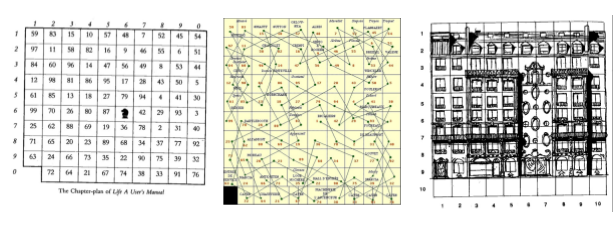
\includegraphics[width=\textwidth]{figures/2-Ice-Bound/calvino-tables.png}
    \caption{The numbered chapters of \textit{Life: A User's Manual} laid out on a grid (left) and the path of the ``knight's tour" comprising their traversal (middle) which describes the story that takes place in the corresponding room in the layout (right) \cite{harding_2014}.}
    \label{fig:calvino-tables}
\end{figure}

%%%%%%%%%%%% END FIGURE %%%%%%%%%%%%%%%%%%%%%%%%%%%%%%%%

Perec then used a ``knight's tour" to traverse the map he had created, a concept that was in vogue within Oulipo at the time. A knight's tour is the path created by moving a knight through a grid while visiting every square (Figure \ref{fig:calvino-tables}). This elaborate system of constraints was created to provide lists of required elements for each chapter. Much like the authoring constraints set up by \textit{Ice-Bound}'s system (whose pragmatics we'll explore in Section \ref{par:pragmatic-tables}), the organization of the thematic system constrains enough that it can actually drive authoring in well-specified ways, though the task may be daunting both in scope, and in the ambitiousness of the coherency of output.

A particularly evocative example of this problem can be seen from Calvino---another Oulipo member---and his engagement with constraint-driven combinatorics. Specifically, his 1973 book \textit{The Castle of Crossed Destinies} engages with a tarot deck to structurally frame two collections of stories \cite{crossed_destinies}. In it he lays out two ``spreads" in the shape of the castle and the tavern, and the vignettes that proceed from the lines of cards are closely tied to the symbols of the cards (Figure \ref{fig:calvino-castle})

%%%%%%%% BEGIN FIGURE %%%%%%%%%%%%%%%%%%%%%%%%%%%%%%%%%

\begin{figure}
    \centering
    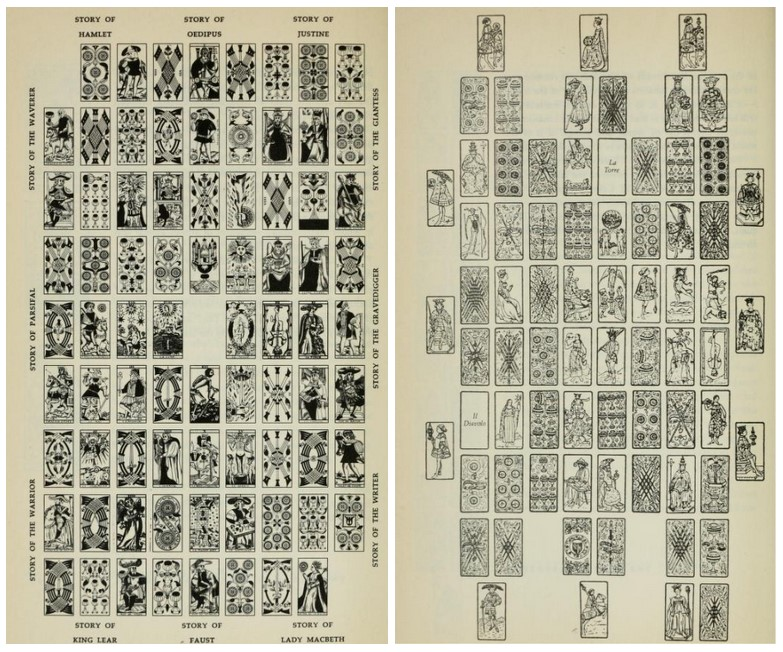
\includegraphics[width=\textwidth]{figures/2-Ice-Bound/castle-of-destinies.jpg}
    \caption{The card layouts for the castle (left) and the tavern (right).}
    \label{fig:calvino-castle}
\end{figure}

%%%%%%%%%%%% END FIGURE %%%%%%%%%%%%%%%%%%%%%%%%%%%%%%%%


While his goal was initially ambitious, the writing of this work proved too daunting and difficult to complete in its purely generative form (accounting for every combination of cards in the layout, with a coherent story for each). Calvino elaborates upon this in the Afterword, where he describes his process: ``I publish this book to be free of it: it has obsessed me for years. I began by trying to line up tarots at random to see if I could read a story in them [...] I looked for other combinations of the same cards; I realized the tarots were a machine for constructing stories." Having realized the generative storytelling potential of the divination deck, potentially ripe with rich and variegated meaning, Calvino was then ``tempted by the diabolical idea of conjuring up all the stories that could be contained in a tarot deck [...] I wanted each of the stories to have a coherent significance."

Calvino's strategies to navigate the generative chaos of combinatorics mirror those used by authors in digital forms. His first approach was to take two existing and well-defined stories---that of \textit{Roland the knight} and \textit{Astolpho}---and pick the tarot cards that would allow him to tell those stories. The rest of the cards he let fall where they may, and told those stories ``as they came." By giving two stories primacy, he was able to chart an easier course through the generative waters, and could excuse discrepancies in the other stories as vagaries of what was necessary to provide the unified structure for the main narratives. He ran into issues however, when---girded perhaps by his success with the tavern section---he was ``unwilling to sacrifice any of the narrative possibilities" for the castle section, and sought something more generative. Practitioners in the field will be well familiar with what resulted: Calvino bemoans how he ``spent whole days taking apart and putting back together my puzzle [...] I drew hundreds of patterns [...] but some essential cards were always left out, and some superfluous ones were always there in the midst. The patterns became so complicated [...] that I myself was lost in them." To escape from this impasse he quite literally gave up on the patterns and instead wrote directly the ``tales that had already taken shape, not concerning myself with whether or not they would find a place in the network of the others." But he was stuck between a rock and a hard place, because without the restraint of the deck, the point of the exercise would be lost. As he says: ``without it, the whole thing was gratuitous."

Calvino also ran into issues with realizing his ``surface text", another familiar problem to practitioners. Though he would successfully come up with a series of cards to use for a story visually, when he began writing them down they would lose their compellingness, and had to be eliminated ``because they would have lowered the tension of the style."

He gave up multiple times, and would then take up the project again later, hoping that a fresh attack ``in a different way, more simple and rapid" would garner success. He spent countless hours shifting and re-aligning symbolic patterns, only to---upon waking the next morning---``tear it up." He never reached a sense of closure with the manuscript, working it over and reformulating it even as the manuscript was in the final stages of publication \cite{crossed_destinies}.

As with previous works we covered, he reflected this dilemma diegetically, such as in The Waverer's Tale, where the Devil card confronts the Waverer and proclaims ``Whoever retraces the way of divided things encounters me, whoever descends to the bottom of contradictions runs into me, whoever mingles again what was separated feels my membraned wing brush his cheek." Also present on the card are two smaller figures on leashes, and Calvino muses that ``it is likewise probably that each of them holds on a leash two other, smaller devils that have remained outside the picture, so that from branch to branch stretches a network of ropes which the wind sways like a great cobweb." A web which resembles the net of correspondances he himself was trapped by in writing the book, although some \cite{conte_1994} have also theorized it was meant to symbolize Borges and his engagement with multiplicity in ``The Garden of Forking Paths."

Calvino set himself a more structured---and therefore perhaps more achievable---goal in 1983 with the novel \textit{Mr. Palomar} \cite{calvino1985mister}. Each section of this work is guided by the constrained combinatorics of three themes partnered with ``kinds of text experience":

\begin{enumerate}
\item Visual (text as pure description)
\item Anthropological / cultural, involving language, meaning, and symbols (text as story)
\item Speculative, concerning cosmos, time, infinity, and the dimensions of the mind (text as  meditation)
\end{enumerate}

The novel is divided up into twenty-seven sections grouped in three levels, each numbered from 1.1.1 to 3.3.3 with every permutation in-between. Therefore, section 1.2.3 would contain an element from each theme/mode category, whereas section 2.3.3 would be lacking in purely descriptive text.

These works, and the thematically constrained writing they provoked, is evocative of the process used for \textit{Ice-Bound}, though our computational processes were more complex. In \textit{Ice-Bound} we determined through early design sessions and testing to use 25 themes (which run the gamut from genre to character traits) for the sake of combinatorics. The ``exercise" of fulfilling the content requirement for that system led us to authoring situations where we would need to write a section with a general mood of horror, with the subject of ``lightning doesn't strike twice," a combination of constraints that perhaps would be familiar to Perec or Calvino. We will revisit and elaborate upon this correspondance in Section \ref{subsubsec:25-themes-and-12-tags}.
%%GDoc comments%%  
% I've now broken these into "non-digital" and "digital" combinatoric works, and expanded the non-digital ones more extensively, while also adding some new sections under the digital works to flesh them out
\subsection{Digital Combinatorial Fiction}\label{subsec:digital-combinatorial-fiction}

Combinatorial narrative really shines, however, when it uses the affordances opened up by computers. Works which normally would be challenging to print or reprint can be translated with ease, such as J.M. Coetzee's digital version of Beckett's \textit{Sans / Lessness} short story consisting of 120 randomly selected sentences \cite{lessness}. But the real benefit comes from the increase in sheer scope computational media affords new works. While enumerating the full breadth and depth of work in digital combinatorial fiction is far beyond the scope of this dissertation, there are some specific categories of works which relate more directly to the specific concerns we had while creating \textit{Ice-Bound}.

\subsubsection{Digital Cards}\label{subsubsec:digital-cards}

One of the most directly related categories of work to \textit{Ice-Bound} revolves around the idea of ``digital cards" as an organizational metaphor. This idea has been around for some time, with a prominent early work being Bernstein's \textit{Card Shark} system which was proposed in 2001 \cite{bernstein_cardshark}. \textit{Card Shark} was a system created to explore the notion of sculptural hypertext, a term Bernstein defined as hyperfiction that is structured ``by removing unwanted connections, much as a sculptor may create objects by removing unwanted material" \cite{bernstein_cardshark}. This was in contrast to what he termed calligraphic hypertext, which begins without links, which the author then creates \cite{bernstein_2007}.This system was not fully developed and used to author works on its own, however the notion of sculptural hypertext was incorporated into StorySpace 3, as an improved authorial affordance on the existing ``guard fields" capability. The ability to add guard fields to lexia is a feature present in StorySpace since its initial versions, as preconditions that could be associated with links between texts. The new functionality added the ability to guard story spaces comprised of several lexia with predicates (called requirements) which could also change the state of the hypertext when certain lexia were visited \cite{bernstein_decline}. This was then used to author a work \textit{Decline and Fall}, to demonstrate the new affordances.

Tarot cards, which so perniciously snared Calvino, have continued to capture the imagination of digital practitioners. Works like Hooper and Weal's 2005 \textit{StorySpinner} system \cite{storyspinner}, directly inspired by Calvino's \textit{Castle of Crossed Destinies}, presents stories based on cards selected by the reader, though Hooper and Weal are careful to specify that they do not consider the system a ``generator of text", but rather a system for organizing narrative segments. However, the generative possibilities it makes possible, through time constraints (certain nodes cannot show up before others), exclusionary logic (barring mutually exclusive events), and a variable rating function with five modes for preference for strict or random structure, means that with appropriate authoring, complex works could be conceivably made. Sullivan et al created a provisional system that creates ``short movie-like story synopses, along with a tagline one might see on a movie poster" in response to generated draws of Tarot cards \cite{sullivan2018tarot}.

However, Tarot can also be generalized as a hierarchical or ontological approach, which applies metaphorically to a body of narrative material to be drawn into juxtaposition in specific ways. The most sophisticated extrapolation of this is Short's \textit{Annals of the Parrigues} \cite{short_annals}, which takes the five top-level categories of Salt, Mushroom, Venom, Beeswax, and Egg, and associates several properties to them. Furthermore, she associates an authoring practice with each category, from the fungal generativity of Markov chains to the ``venomously written", hyper-targeted generative grammars. 

%%%%%%%% BEGIN FIGURE %%%%%%%%%%%%%%%%%%%%%%%%%%%%%%%%%

\begin{figure}
    \centering
    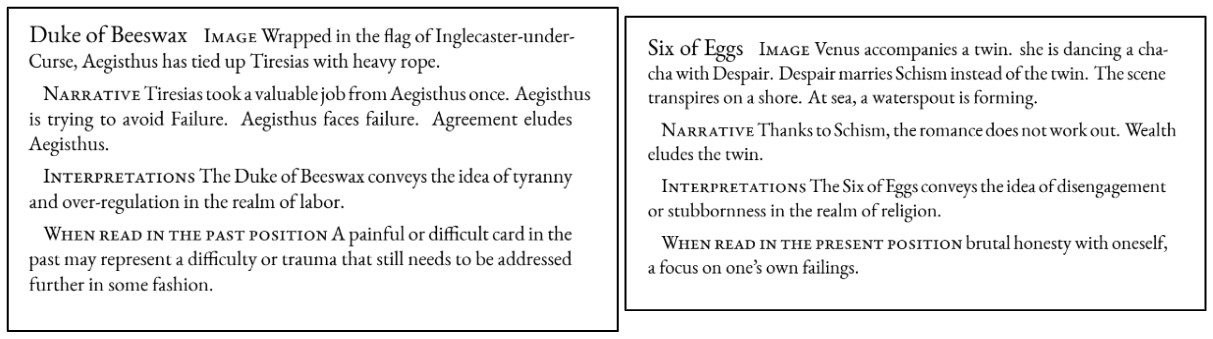
\includegraphics[width=\textwidth]{figures/2-Ice-Bound/parrigues.jpg}
    \caption{Two sample cards from the \textit{Tarot of the Parrigues}.}
    \label{fig:parrigues}
\end{figure}

%%%%%%%%%%%% END FIGURE %%%%%%%%%%%%%%%%%%%%%%%%%%%%%%%%

\textit{Annals of the Parrigues} is a static, non-interactive document, dynamically generated in participation with Kazemi's 2015 ``NaNoGenMo" (National Novel Generation Month) celebration \cite{kazemi_2015}. Short later developed the same system further to create the \textit{Tarot of the Parrigues}, which dynamically generates a Tarot-like deck. The design process iteratively progressed in development through n-gram word association, narrative arc generation, quality control through custom metrics, and custom tagging which allowed for increased narrative causality. The result was cards which contain text descriptions of characters of the \textit{Parrigues}, a brief narrative segment of an event they describe, along with a suggested interpretation (Figure \ref{fig:parrigues}).

These systems again take up the mantle of interlocking thematic constraint, although this time engaging in a sort of meta-combinatorics, generating collections of cards which themselves have a sub-possibility space of potential combinations and expressions.

But beyond generation of cards themselves, we can turn to the more structural, narrative qualities of what kinds of stories systems can enable us to tell. Two main approaches are most relevant to \textit{Ice-Bound}, quality-based narrative systems, and salience-based narrative systems.
%%GDoc comments%% 
\subsubsection{Failbetter and Quality-based Narrative Systems}\label{subsubsec:failbetter-and-qbn-systems}

Failbetter Games is a relatively small indie studio based out of London, known for their flagship game \textit{Fallen London} (first released in 2009) and their more recent games \textit{Sunless Seas} (released in 2015) and \textit{Sunless Skies} (released in 2019). \textit{Ice-Bound}'s development (2013-2016) made it contemporaries with \textit{Fallen London} and Failbetter's StoryNexus engine. 

StoryNexus was the core of \textit{Fallen London}, and was also freely available for people to use to author their own narratives. It had a web-based interface similar to modern Twine, but unlike Twine, possessed an integrated website / marketplace where people could browse and read narratives written with it. This web-based authoring system enabled the creation of what Failbetter calls ``quality-based narratives." These narratives are composed of ``storylets," which Failbetter characterized as ``discrete chunks of narrative that can be played in any order, as many times as you like" \cite{arendt_structuresOne}. These storylets are essentially small pieces of story content bounded by pre-conditions and post-conditions (effects). They each have one or more ``branches" which are the choices made available to the player. Each branch has ``results", which modify qualities. Results can also vary based on success or failure, allowing players to pass or fail ``quality checks." In terms of narrative design, storylets are encountered singly, or in larger interconnected structures called ``Ventures," which are gated and driven by the quality state of the player \cite{ifwiki_2019}.

Qualities are essentially stats. They might be an integer for how many nightmares one has had, a flag for whether a particular storylet has been visited, etc. It's a simple blackboard system, but the design work that goes into Failbetter stories is what makes it really shine, and brings out its complexity.

StoryNexus narratives have some core design assumptions gathered around the metaphor of a card deck. The player has a hand, which can contain a certain number of cards, and an ``Opportunity Deck", which contains a certain number of cards, which can fluctuate wildly in the course of the game depending on the player's qualities, location, or setting (a fact Failbetter narrative designers must anticipate and account for).

Also central to the StoryNexus platform is the concept of ``actions", which are a limited resource, and used every time the player takes an action. They refresh over time, which provides authors a way to meter out and also monetize their content (the two primary ways being ``expansion pack stories" and ``purchase more actions"). It's an interesting platform decision, as it means it is not possible to play through \textit{Fallen London} in one, or even several, playthroughs. This design is ``baked into the content and pacing" such that moving it away from that model would take an estimated 20-25 months of effort on their part \cite{failbetter_ftp}. Some of this presumably is based on the fact that a category of card triggers in StoryNexus games are time-based, but there may be other aesthetic considerations at play as well.

The ability of these stories---told through a series of connected vignettes---to communicate a coherent narrative relies on a design consideration Failbetter calls ``implicit storytelling" or ``fires in the desert." The metaphor is that one imagines the player wandering a dark desert between campfires---we don't need to specify how they got from campfire to campfire. The player can fill in that blank on their own. This design ethos generalizes structurally to the combinatorial nature of the experienced narrative, where storylets may happen in several different potential orders, which doesn't cause problems if the player is given the tools to bridge those gaps on their own. One of Failbetter's founders characterized this approach as making Failbetter games ``a montage: we provide the shots, the player does the arrangement" \cite{arendt_structuresThree}.

\textit{Fallen London} is an immensely successful combinatorial narrative. It is also a very large combinatorial narrative. Conservatively, there are more than 2000 root-level storylets \cite{fallen_london_wiki}, not counting the associated content for each of a player's available choice options and outcomes for each one (which their authoring guide broadly suggests should number around five per storylet). The total word count is in the neighborhood of 1.5 million words \cite{failbetter_ftp}, spread between a team of several authors. This sort of undertaking demands rigorous systemic design knowledge and practices in order to make authoring tenable.

Due in part also to StoryNexus being a platform and public community of practice, Failbetter was motivated to formalize and make public several authoring patterns and design practices they used in crafting their combinatorial narratives. There are more than 60 different authoring patterns, split between content design \cite{storyChoices_contentDesign}, branch design \cite{storychoices_branchDesign}, and choice design \cite{storyChoices_choiceDesign} (although these distinctions overlap and can be somewhat muddy). Some examples can be seen in Figure \ref{fig:storynexus-patterns}.


%%%%%%%% BEGIN FIGURE %%%%%%%%%%%%%%%%%%%%%%%%%%%%%%%%%

\begin{figure}
    \centering
    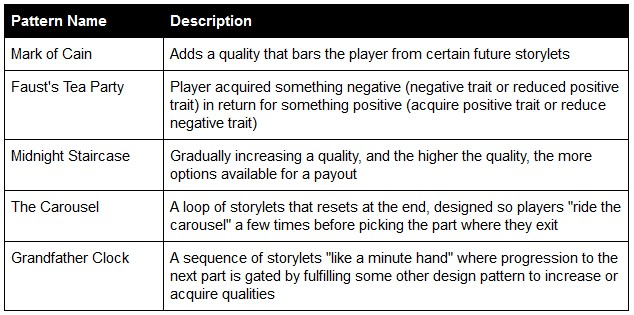
\includegraphics[width=\textwidth]{figures/2-Ice-Bound/storynexus-patterns.jpg}
    \caption{A selection of StoryNexus authoring patterns.}
    \label{fig:storynexus-patterns}
\end{figure}

%%%%%%%%%%%% END FIGURE %%%%%%%%%%%%%%%%%%%%%%%%%%%%%%%%

These authoring patterns were intended to be used in specific, grounded cases, but there is also some generalized design advice for authoring with StoryNexus. Most salient to our pursuit of practices increasing authorial leverage is Failbetter's notion of ``quality parsimony."

Quality parsimony means reducing the number of unique entries into the state blackboard (qualities) as much as possible during the design/authoring process. This simple rule has some long-reaching structural effects. Failbetter opted for this type of narrative design instead of a more traditional branching pattern, wanting their stories to structurally resemble more ``a river rather than a tree [...] You want any one character [here meaning the player] to see 90\% of your content, not 50\% or 10\%" \cite{arendt_structuresThree}. One could see this mapping to the Authorial Leverage framework as wanting to increase authorial Clarity, such that---as the number of storylets grows---there isn't a concomitant growth of the blackboard state such that it  becomes untenable for authors to easily hold it in their mind as they plan and write future Ventures.

The hours poured into design resources and documentation of StoryNexus enabled a rich and varied community, with large and elaborate combinatorial narratives that afforded writers with little programming background the ability to create procedural stories, and even monetize their efforts. This lead to amazingly complex and baroque works (quality parsimony aside) such as \textit{Black Crown} by Rob Sherman, which engaged with the unique limitations of the StoryNexus platform (such as the limit to player actions) as diegetic material arising from its fictional world \cite{reed_blackCrown}.

StoryNexus as a platform, unfortunately, did not prove to be sustainable over a long period of time. Even with support from Random House, projects like \textit{Black Crown}---with their concomitant ``unique features and separate, demanding bug queue" \cite{sherman_2014}---proved too unwieldy, and the labor required to support them untenable. StoryNexus was officially shuttered near the end of 2013 due to the monetization of the platform being insufficient to support platform maintenance and development. Failbetter had just successfully run a Kickstarter for their new property \textit{Sunless Sea}, and decided to consolidate their efforts around developing and launching that game in the new modality, leaving StoryNexus as an archival body of community-authored work in testament to the early system \cite{kennedy_2013}.

\paragraph{Similarities and Differences.}\label{par:storynexus-similarities-and-differences}

While the combinatorial nature of StoryNexus's system was definitely something similar to what we wanted in terms of \textit{Ice-Bound}'s dynamics, a big difference was that we wanted the experience of an \textit{Ice-Bound} level to be more about exploring a narrative possibility space through quickly making easily-reversible choices. The feeling we were trying to capture was more an editorial one, or as Reed put it, a ``sculptural" one. This meant that, unlike StoryNexus games which hinge around the idea of progress through a series of choices that can occur in different orders, but which permanently affect the state space, we wanted a game where many ``choices" could be made and reversed, until the player had a path through the story they were satisfied with. While the systems under the hood might have some similarities, it is this key difference that distinguishes the \textit{Ice-Bound} system and approach from StoryNexus games. Additionally, we wanted players to be able to make as many changes as they wanted, unmetered and unlimited, as opposed to StoryNexus's approach with their actions.
%%GDoc comments%%
\subsubsection{Salience-Based Narrative}\label{subsubsec:salience-based-narrative}

This sort of experience architecture, where content is selected based on underlying qualities driven by player interaction, has a close cousin. If we consider instead that the system is evaluating player input and state, in order to \textit{automatically} select the most salient content to display, we can use the lens of what Short calls ``salience-based narrative" \cite{short_salience}. The heuristics driving content selection can be very simple, yet create compelling experiences when supported by proper design.

A good example of this can be seen in Barlow's \textit{Her Story} \cite{barlowe_her_story} and \textit{Telling Lies} \cite{barlowe_telling_lies}, two narrative games whose only interaction is through entering database queries to different short film segments. In \textit{Her Story} these are recordings from a police office as they interview suspects for a murder. In \textit{Telling Lies}, the videos are one-way recordings of characters' webcam input, forcing the player to try to piece together the story's dialogues across clips.

For both, the player's interaction is restricted to entering text queries into a diegetic search engine. The game then goes through the library of content, and presents video clips that match (Figure \ref{fig:barlow}). While this is deceptively simple, the finesse of the experience is wholly in the design of the interface and the manner in which the videos are tagged. For example, in both experiences only five video results will be displayed, even for terms which have more than five results. Thus, the reader's strategy of finding content evolves very quickly from queries like ``murder" to more specific ones referencing information they've gleaned from more general clips. Also, the tagging itself is a mixture of thematic and keyword-driven excerpts from the clip transcripts.

%%%%%%%% BEGIN FIGURE %%%%%%%%%%%%%%%%%%%%%%%%%%%%%%%%%

\begin{figure}
    \centering
    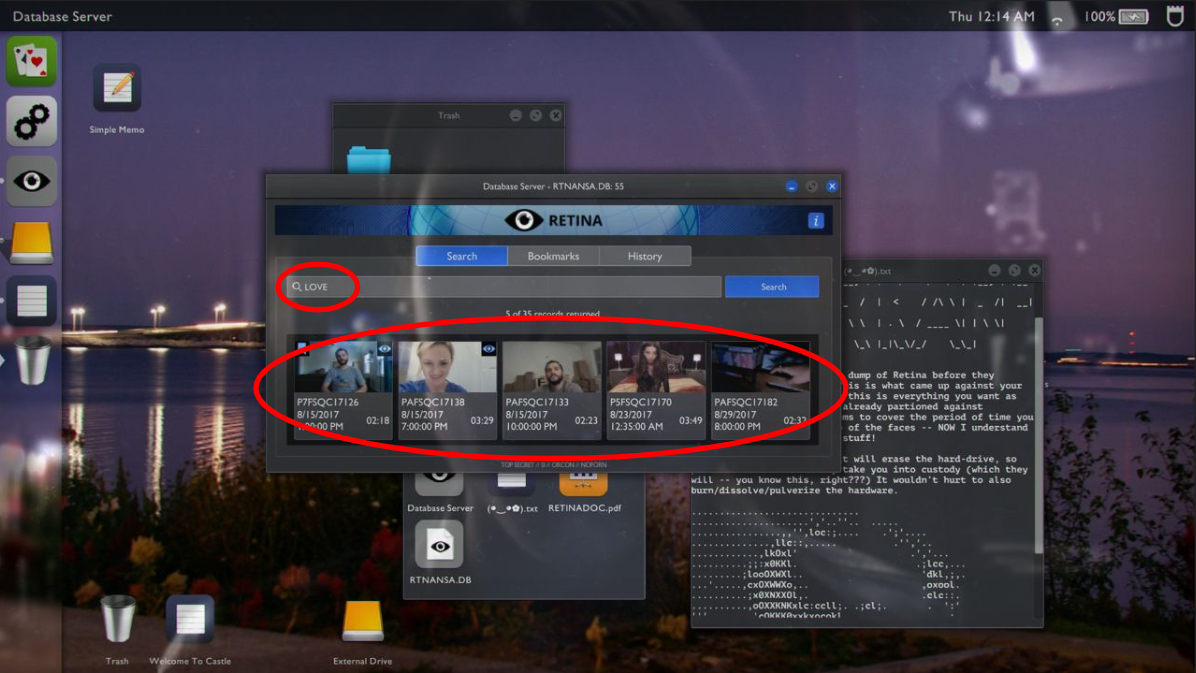
\includegraphics[width=\textwidth]{figures/2-Ice-Bound/barlow.png}
    \caption{A screenshot from Telling Lies, with the search term ``LOVE" circled, and the resulting five video clips that match that term circled.}
    \label{fig:barlow}
\end{figure}

%%%%%%%%%%%% END FIGURE %%%%%%%%%%%%%%%%%%%%%%%%%%%%%%%%

Barlow has skillfully designed a database such that, because one can only know terms after watching certain clips (such as the importance of the suspect's guitar in \textit{Her Story}) the available exploration pattern---discounting pure luck---could be viewed as a choice-driven tree structure, where each ``choice" is one of the clips brought up in the query.

Of course, more complex tagging examples exist. The prevalence of tag- and trigger-driven content has been around in first-person style games for quite some time. One more recent example that is especially colorful is the indie game \textit{Firewatch}. In it, the player takes on the role of Henry, a ranger who's been assigned to a fire watchtower for the summer. The bulk of the game's content comes from communication through a handheld walkie-talkie and radio with Delilah, a fellow ranger stationed in the neighboring tower.

What makes this interesting is that the conversations for \textit{Firewatch} are all contextually triggered by actions the player takes in the game. As noted in a Slate interview with Vanaman, Firewatch's main writer:

\begin{quote}
"The conversation is putting itself together dynamically, and that means it can be hyper-specific,” said Vanaman. “There are 10,000 events in the game—speech and everything else—that can happen.” Rather than simply shunting you from branch to branch of a dialogue tree, the game looks at everything you’ve said and done, and picks the truest and most specific thing that can happen next. “There are so many [variables] in our game that are so silly and weird. There’s stuff like, has Henry ever mentioned the outhouse? Maybe that matters." \cite{hudson_2016}    
\end{quote}

\paragraph{Similarities and Differences.}\label{par:salience-similarities-and-differences}
In a way, the pre-condition logic \textit{Ice-Bound} uses for determining what content to show bears similarity to the design methodology for salience-based narratives. On a code and general software architecture level, we're reacting to player actions, and determining the ``most salient" content to display. However, from a design perspective, the pre-condition logic is much more geared around narrative coherence with what the player has chosen to make active in the story, as opposed to reactive to diegetic actions the player may take in a story world. And while the use of continuous thematic context (discussed in Section \ref{subsubsec:25-themes-and-12-tags}) allows for a similar experience to Barlowe's use of progressively specific keyword tagging, we leverage that in a more systemic way for \textit{Ice-Bound}'s finale (discussed in Section \ref{subsubsec:thematic-finale}).
%%GDoc comments%%
\subsubsection{\textit{King of Dragon Pass} and \textit{Six Ages}}\label{subsubsec:king-of-dragon-pass}

Another game in dialog with \textit{Ice-Bound} is David Dunham's \textit{King of Dragon Pass}, first released in 1999, but ported twelve years later in 2011 to iOS. Dunham himself provided a nicely succinct description of his game \cite{dunham_2011}, saying it

\begin{quote}
essentially has an underlying resource management game which serves as the skeleton that supports the stories. [...] Play consists of alternating resource-related actions, and responding to story scenes. These consist of an illustrated situation, usually with five choices. These may lead to secondary choices, but still within the same situation, until it’s resolved. Resolution may have specific later consequences, but typically influences the economic model of the resource management game. Parts of the story and setting are actually revealed through your advisors, individuals you pick to sit on the clan council. While you can lose the game through poor resource management (or bad luck), you can only win by story choices.    
\end{quote}

In contrast to StoryNexus games, \textit{King of Dragon Pass} and \textit{Six Ages} both obscure the ``qualities" driving the logic of different scenes, a decision Dunham said was made out of a desire to prevent the presence of statistics from ``breaking the fantasy" of the world. Additionally, he admitted to randomness playing a larger part as well, compared to the more deterministic combinatorial paths through the multitudinous decks of StoryNexus works.

\textit{King of Dragon Pass} conforms as well to the same ``choice metric" Failbetter suggests, with five choices per ``scene" if possible. Dunham keeps runaway content contained by limiting these scenes to one or two choices, after which the stats are adjusted, and play continues in the simulation. This sort of modular design keeps the chances of unforseen long-term combinations or effects from sabotaging gameplay. 

\textit{King of Dragon Pass} sports 500 events, which makes the pool smaller than Failbetter's games, though it is still more than enough to incur substantial authorial burden, especially when taken into consideration with the potential knock-on effects from the simulation system running alongside it, including both an economy and a social model. Additionally, the simulation allows different ``modes" of player actions---such as sending a caravan or setting ratios of crafting quality---which have a more systemic effect than the more atomic actions players take in StoryNexus games \cite{dunham_repeatability}. While events may repeat, it will typically be a substantial period of time before they do, and Dunham relies on the context of the event's recurrence changing the encounter enough that it retains its interest.

This event dynamism comes by virtue of the DSL (domain specific language) Dunham created for \textit{King of Dragon Pass}, and later elaborated upon for \textit{Six Ages}. OSL (Opal Scripting Language) is meant to be more approachable for the writer than coding in C++, the language both were originally written in. OSL affords dynamic character casting, so that recurring events can star the same characters, or characters can be cast by trait. It also allows randomized or trait-dependent text display, which---when paired with pre-condition logic checks for traits---keeps events salient to your decisions as the game progresses \cite{dunham_2008}.

\paragraph{Similarities and Differences.}\label{par:dragon-pass-similarities-and-differencs}
\textit{Ice-Bound} shares storytelling approaches with the system in \textit{King of Dragon Pass}---we similarly wanted to have self-contained vignettes gated by pre-conditions, and use a simple blackboard structure to drive that. However, as with our difference from StoryNexus, we wanted to pursue a mode of interaction that was more about continuous editing and undoing of changes, to give a more exploratory feel. \textit{Ice-Bound} also makes use of character casting for its components, which adds to the dynamism of scenes. Also, we had no desire to impart any kind of simulation to the game, which \textit{King of Dragon Pass} uses in concert with its narrative to drive the experience. The ``window into procedurality" we wanted to provide was rather through exposing the conditions themselves, so that---unlike Dunham's position that knowing underlying state variables breaks the fiction---players know exactly the reason content displays, and can use that to further enrich their strategies for exploration.


\section{Relationship to Related Works}\label{sec:ice-bound-relationship-to-related-works}

Situated in dialogue with this body of combinatorial narrative, \textit{Ice-Bound}'s development was uniquely positioned to offer an experience geared around enabling the reader to make low-friction, frequent changes to a narrative possibility space, coupled with vignettes of a substantial length with high quality surface text, yet still causally connected via their pre-condition logic. The incorporation of conversations with a character using more traditional branching choice structures injected a note of familiarity, and the incorporation of material into a printed book provided a more ``static traditional medium" to convey longer pieces of the story.

\section{System Description}\label{sec:ice-bound-system-description}

\subsection{Summary}\label{subsec:ice-bound-summary}

\textit{Ice-Bound} consists of three systems, two of which operate primarily as a support for the central one. The central system is a combinatorial narrative system (Figure \ref{fig:ice-bound-system}), which drives the main narrative. This is supported by a tag-based content selection system (used when scanning pages from the book) and a branching dialogue system (used for dialogues with the character KRIS).

%%%%%%%% BEGIN FIGURE %%%%%%%%%%%%%%%%%%%%%%%%%%%%%%%%%

\begin{figure}
    \centering
    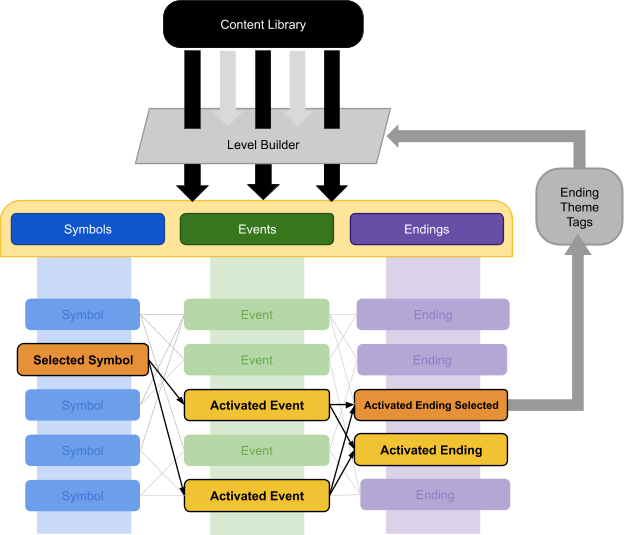
\includegraphics[width=\textwidth]{figures/2-Ice-Bound/ice-bound-system-diagram.png}
    \caption{A diagram of the flow in the combinatorial narrative system. Content is filtered and selected through the Level Builder. Valid symbols, events, and endings are displayed. The player then selects whatever symbols they desire, which in turn activate events, which in turn activate endings. When the reader is satisfied with a given set of activated symbols, events, and an ending, they select the ending. The thematic tags of that ending are then added to the filter logic of the Level Builder, the next level's content is selected, and the cycle begins again.}
    \label{fig:ice-bound-system}
\end{figure}

%%%%%%%%%%%% END FIGURE %%%%%%%%%%%%%%%%%%%%%%%%%%%%%%%%

\subsubsection{Combinatorial Narrative System}\label{subsubsec:combinatorial-narrative-system}

The main \textit{Ice-Bound} game interface is ``blueprint mode" (Figure \ref{fig:blueprint}), which shows a blueprint-style overview of the current level's rooms. Each room has some number of sockets (the ``cigar box" or ``round table" in Figure \ref{fig:blueprint}), each of which is tied to a particular symbol card. Each level, the player is provided some amount of ``light", symbolized by glowing yellow circles, that they can drag around onto sockets to activate the symbol cards.

There are three types of cards in the system: symbols, events, and endings. The player can directly activate or deactivate symbols by moving the light. Combinations of activated symbols in turn activate or deactivate events, and combinations of activated symbols and events in turn activate endings.

%%%%%%%% BEGIN FIGURE %%%%%%%%%%%%%%%%%%%%%%%%%%%%%%%%%

\begin{figure}
    \centering
    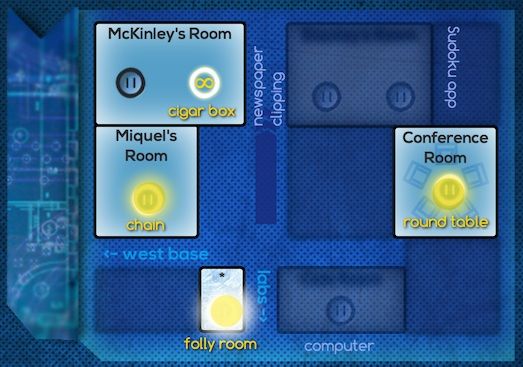
\includegraphics[width=10cm]{figures/2-Ice-Bound/blueprint.jpg}
    \caption{The blueprint UI of an \textit{Ice-Bound} level, showing sockets in rooms. Here we see ``chain", ``folly room" and ``round table" are activated, ``cigar box" is always activated, and ``computer" etc are not activated.}
    \label{fig:blueprint}
\end{figure}

%%%%%%%%%%%% END FIGURE %%%%%%%%%%%%%%%%%%%%%%%%%%%%%%%%

These linkages are established through an authoring convention of content tagging, and simple propositional logic. Most event and ending conditions are based on whether certain symbols or events are active, or symbols and events with particular tags are active. More specific system details will be elaborated on in Section \ref{subsubsec:icebound-complexity}'s discussion of Complexity.

\subsubsection{Tag-based Content Selection System}\label{subsubsec:tag-based-content-selection-system}

When a player has activated symbols such that the resulting story is one they are happy with, they're asked by KRIS to ``confirm he would write something like this" by scanning a page from the book that matches the ending's theme.

\textit{Ice-Bound} uses marker-based augmented reality tracking, so that when the scan mode is activated, players can point the camera of their iPad or computer at the book, and images will display on the pages, revealing further narrative details, or providing some piece of context for how they fit into KRIS's life. The book's format provided us with a chance to write longer story sections, which stood in contrast to the more generative, vignette-like narrative of the digital game. 

Each page in the \textit{Ice-Bound Compendium} is tagged with some number of thematic tags. In contrast to the symbols, events, and endings, these tags are invisible to the reader, prompting a sort of ``thematic scavenger hunt" to find a page which fits the ending selected by the reader. These hidden tags for each page drive recurrent threads or themes throughout the book, but there isn't a set or canonical order to the pages. One might follow the thread of Kris's relationship with his daughter by finding pages scattered throughout detailing its deterioration across multiple themes, but the arrangement of pages was more to provide an equal distribution of tags than any sort of chronology. This was done in order to encourage players to flip through it at length, and reinforced the ``editorial" mode of searching in a body of content for specific evidence to fit a particular narrative.

\subsubsection{Branching Dialogue System}\label{subsubsec:branching-dialogue-system}

%%%%%%%% BEGIN FIGURE %%%%%%%%%%%%%%%%%%%%%%%%%%%%%%%%%

\begin{figure}
    \centering
    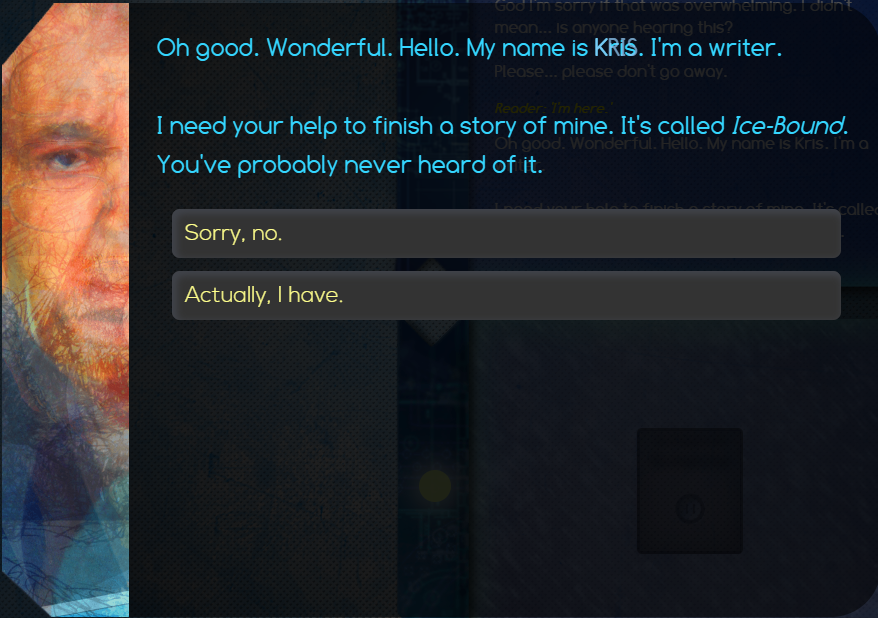
\includegraphics[width=10cm]{figures/2-Ice-Bound/kris-dialogue.png}
    \caption{A screenshot of the dialog system in \textit{Ice-Bound}, where the reader would experience traditional choice-based narrative segments.}
    \label{fig:kris}
\end{figure}

%%%%%%%%%%%% END FIGURE %%%%%%%%%%%%%%%%%%%%%%%%%%%%%%%%


Part of \textit{Ice-Bound} is also talking with KRIS via pop-up branching dialogues. These are done in the usual manner of branching dialogue, where content is authored with links to other content, and the responses the player clicks are their replies to the content displayed. These dialogues have their own state-driven conditions and effects, which allowed us to author dialogues that only appear if symbols with certain tags are activated, or a specific symbol is activated. Combined with state-sensitive templating, this means we could write dialogues with KRIS that leverage the current context of the narrative the player is crafting with great specificity, while still advancing a fairly linear narrative of KRIS's background, and how he was created. The experience this enables is one where KRIS feels like a collaborator who is sensitive to the changes you are making to the story, and that particular context sensitivity is a critical part of communicating that the system is "listening" to the choices the player is making, and that those choices have meaning.

\subsubsection{State-driven Templating and Shimmertext}\label{subsubsec:state-driven-templating-and-shimmertext}

%%%%%%%% BEGIN FIGURE %%%%%%%%%%%%%%%%%%%%%%%%%%%%%%%%%

\begin{figure}
    \centering
    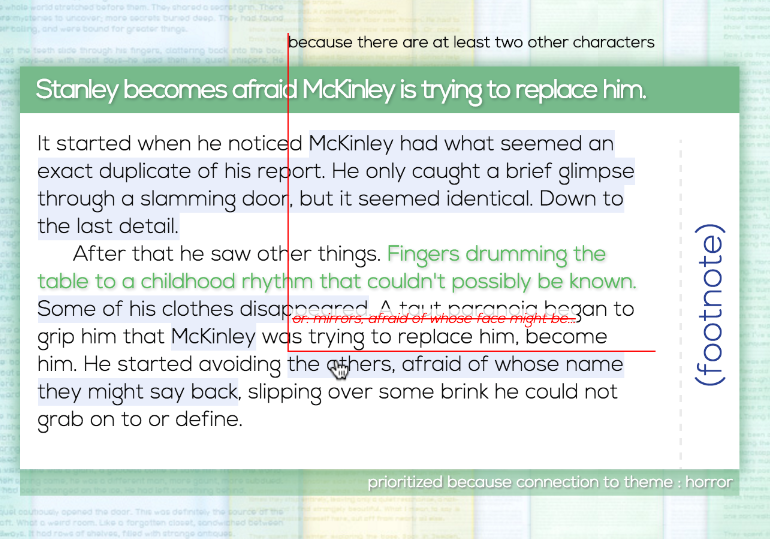
\includegraphics[width=\textwidth]{figures/2-Ice-Bound/event.png}
    \caption{An event in the longer-form portrait-view interface. Note the dynamic text (``McKinley had what seemed an exact…") the shimmertext (``Fingers drumming the table…"), the tooltip-style explanations (``because there are at least two other characters") and the theme trigger text in the bottom right (``prioritized because connection to theme: horror"). The ``footnote", when clicked, starts a KRIS dialogue.}
    \label{fig:event}
\end{figure}

%%%%%%%%%%%% END FIGURE %%%%%%%%%%%%%%%%%%%%%%%%%%%%%%%%


All three systems make use of state-driven templating to change their surface text---sometimes substantially---in order to increase relational cohesion through the different pieces of content displayed to the reader. These were used to keep character casting coherent between fragments, so that the protagonist and antagonist in one fragment would be the same in the next, as well as to bring in key pieces to reinforce flavor from an earlier fragment.

We also made heavy use of ``shimmertext", which is text that shifts between different options continuously. This text styling is supposed to represent places of the story KRIS isn't ``sure about", and the player can help resolve them by tapping on them. Tapping once solidifies the text so it stops shifting, and subsequent tapping cycles the text between its different options. This was a handy catch-all for situations where we wanted to write state-dependent or ``sensible" variation for text, but didn't want to commit to tracking it in the blackboard state or bogging down the pre-conditions. We would simply write the options as ``shimmertext", and rely on the reader to exercise their editorial control to resolve them ``sensibly." Or not! Some players enjoyed the spice of mystery injected into a scene if a character suddenly grimaced at happy news, or seemed happy at misfortune. The fictive framing for this was that it was a shortcoming of KRIS as an artificial entity if they didn't match up, a framing we intentionally leaned into so that, even if the system fell short, it was still a diegetic failure, and not a fiction-breaking one.

\subsubsection{Why the System Works}\label{subsubsec:why-the-system-works}

From a storytelling perspective, \textit{Ice-Bound} makes use of a few ``tricks" to get around some of the pernicious problems with story generation.

As mentioned earlier, we leveraged StoryNexus's design concept of implicit storytelling or ``fires in the desert" \cite{arendt_structuresThree}. As storytellers, we don't need to concern ourselves with what happens between the campfires. The reader can fill in those details, or imagine logically what happens for the character to move between the fires. Scott McCloud had a similar concept called ``blood in the gutter" \cite{mccloud_1994} to refer to action that happens between the panels in the comic. These are narratological leaps the reader is willing to make, ones which, if elided, don't cause too big a disjunct in the reader's model of the story, and can be safely left unspoken. Another way to formulate this is Murray's concept of narrative ``anticipation" and ``dramatic compression." Simply put: as long as the fragments we show the reader shore up and advance the characters or play into narrative conventions, the reader can abstract the rest of the scaffolding necessary to make them sensible \cite{murray_compression}.

Our initial prototype had the player moving between rooms, moving objects, and in general had a more simulationist bent. What we found, though, was that the demands of simulation were moving us further and further away from what we had started out in the project to do: tell a complex, compelling story. After bumping up against simulation complexity when proposing a new part of the story, we decided to shift the design away from that, and let the reader connect the dots themselves. We also didn't want to focus too much on what was ``logical" and therefore ``allowed" in the story, if that meant stifling the player's agency.

The templating system therefore, provided just enough dynamism to keep the campfires in sight, so to speak. Our fictional framing---that the story was riddled with errors and bad drafts---also helped ``frame the failure" such that when our system fell down, we could rely on the player to move away from those mistakes, and even to see them as aesthetic choices we had made \cite{reed2014ice}. As noted earlier, this cohesion bolstering was also accomplished by using shimmertext when we weren't sure or didn't have time to model dependencies for certain sentences or words within sentences. The important thing is that the core causality for these events was preserved as they flowed to create a story for the chapter.

In the course of writing and testing, we found anecdotally that mismatches between time and location were fine, because players would assume a subsequent scene took place later, or was a flashback. More problematic would be when player qualities or emotions didn't seem to match up, where a character's reaction to one event when it happened was anger, but in a later event referencing it, the character was said to have been happy. This led us in writing the cards to craft pieces of story that were relatively self-contained, but had a few tendrils here and there reaching out, usually in the context of their theme or themes.

\subsubsection{25 Themes and 12 Tags}\label{subsubsec:25-themes-and-12-tags}

\textit{Ice-Bound}'s narrative design also makes use of tagging in various ways to provide consistency, and heighten the sense of responsiveness in the system over time.

%%%%%%%% BEGIN FIGURE %%%%%%%%%%%%%%%%%%%%%%%%%%%%%%%%%

\begin{figure}
    \centering
    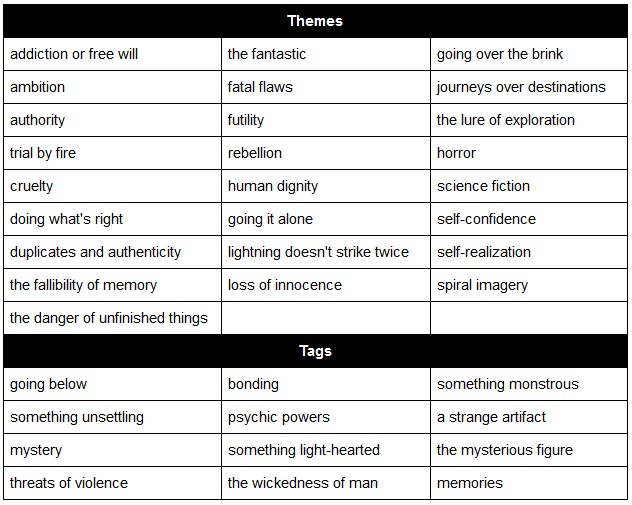
\includegraphics[width=\textwidth]{figures/2-Ice-Bound/themes-and-tags.jpg}
    \caption{Themes and tags used in \textit{Ice-Bound}.}
    \label{fig:themes-and-tags}
\end{figure}

%%%%%%%%%%%% END FIGURE %%%%%%%%%%%%%%%%%%%%%%%%%%%%%%%%

In the course of creating the story, we categorized content broadly into 25 themes. Each piece of content, whether it was a symbol, event, or ending, could have two or three themes applied to it. This was used mainly for the triggering logic between them, so that we could target broad categories of content when necessary. However, it also had another use.

When the player confirms an ending that they think is best, find it in the book, and scan it in using AR, KRIS has a dialogue with them about the page. Each page has roughly three to five themes, and he asks the player which one of them they were thinking of primarily. When the player makes their suggestion, KRIS then picks another theme on the page as one he ``likes" as well.

When the next level is generated, the symbols selected to populate it take into account the themes the player has selected. This means that, as the player continues in \textit{Ice-Bound}, they can end up with stories that cleave closer to the type of content they want to see. Sometimes these differences can be quite noticeable, in the case of more obvious themes like ``science fiction" or ``horror."

\subsubsection{Thematic Finale}\label{subsubsec:thematic-finale}

We wanted to do something special for the finale of \textit{Ice-Bound}, something that would show that all the choices the player had been making along the way had been building towards something. More than anything, we wanted to avoid a situation where the player felt that the ending was ``pre-baked" and only had slight differences depending on their choices. However, we also didn't want to commit to something that would put undue burden on us, such as a wholly new system or mechanic. And we didn't want to commit to a lot of custom authoring, which would most likely never be seen by most players, given the relatively low completion rate of \textit{Ice-Bound} playthroughs as a whole.

%%%%%%%% BEGIN FIGURE %%%%%%%%%%%%%%%%%%%%%%%%%%%%%%%%%

\begin{figure}
    \centering
    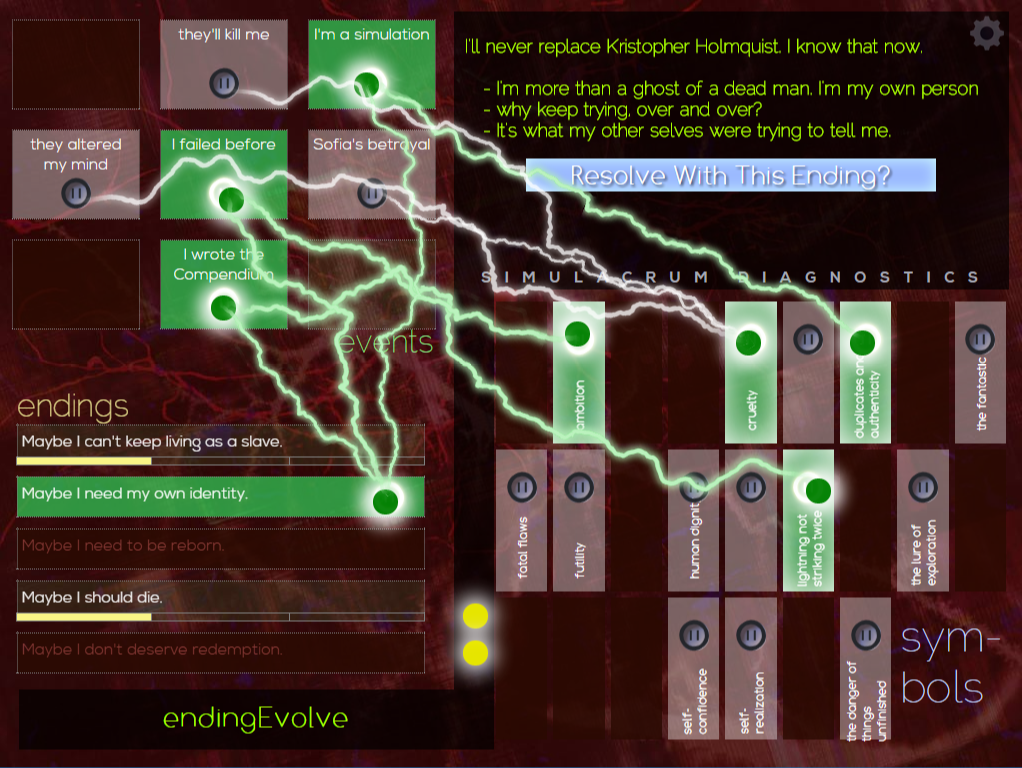
\includegraphics[width=\textwidth]{figures/2-Ice-Bound/finale.png}
    \caption{The final level. The player still drags lights onto symbols (which are now themes) which activate ``events" (KRIS's self-realizations) whose text is in the upper left (``why keep trying, over and over?") and when all three required events are activated, the ending lights up (``Maybe I need my own identity").}
    \label{fig:finale}
\end{figure}

%%%%%%%%%%%% END FIGURE %%%%%%%%%%%%%%%%%%%%%%%%%%%%%%%%

Our solution was to use the themes players (and KRIS) activated in the course of their playthrough as the ``symbols" for the final level. The story of this level is the story of KRIS's life---the justification for the ending action he will take, which can range from escape to self-destruction. In a manner now familiar to players, they drag the lights to activate the themes, which ``electrify" to activate the ``events." In this case the events are more ``justifications" for the action KRIS will take, drawn from information the player uncovered through the course of play, and re-contextualized as justifying a particular action (in Figure \ref{fig:finale} it's ``I'll never replace Kristopher Holmquist”). When all three associated justifications for an action are activated, the ending is unlocked. In Figure \ref{fig:finale} we can see it is ``Maybe I need my own identity."

Because the combinatorics of this play into the same content production flow as earlier levels, there was very little extra code needed to produce this finale. And because the materials are drawn from the symbols and secrets the player has uncovered through their play, it feels customized and unique. Selecting the ending action plays out one of five final custom branching dialogues with KRIS, which also makes use of templating to change the surface text details to match the particular combination used to activate it.

\section{The Question of Authorial Leverage}\label{sec:the-question-of-authorial-leverage}

\subsection{Traversability}\label{subsec:icebound-traversability}
In order to understand the tool support and design decisions made to tackle the authoring task the experience required, we need to first understand the quality of the space fulfilled by the system. This is the question of Traversability, which breaks down into three sub-questions: Explorability (how much content the player can see per playthrough), Replayability (how much of the content is seen by the player in one playthrough, and how many playthroughs is the player expected to undertake) and Reusability (how often content can be reused).

We will tackle each of these in turn. Having done that, we will be well-positioned to detail the different strategies to address the space they describe, in the following section on Authorability.



\subsubsection{Explorability}\label{subsubsec:icebound-explorability}

One of \textit{Ice-Bound}'s strengths lies in the broadly explorable space it provides its players. This was necessary to provide a player experience as one of ``sculptural fiction" (making many low-risk, reversible choices). This is accomplished through a high degree of variability: each socket in a level can be potentially cast with different symbols (although the pool of valid symbols to draw on differs case-to-case). For example, in the third level in the game---about mid-way through the experience---there are technically around 50,000 different combinations of symbols that can be activated, depending on which themes have been strengthened in the previous levels.

That's a large number! But in terms of \textit{meaningfully different} combinatorics, the sets of activated content that feel qualitatively different is smaller, especially given events are typically triggered by tags or themes, which are much more coarsely-grained groups. As mentioned earlier, there are 37 themes/tags content can be tagged with. However, a piece of content can have many tags, thus flexibly collapsing the combinatorics given the discretion of the author. For example, if we authored three pieces of content each tagged with twelve themes, effectively we’re only dealing with combinatorics of three “groups” of tags.  The number of tags per-content piece fluctuates greatly, but in general we would have around three to five themes per symbol. This still means a very broad array of possible content can present itself, especially given that an activated symbol could not only trigger new events (and thus new stories) but also impart qualities to characters, who may be in multiple pieces of content. For example, activating a symbol like ``borrowedKnife" flags the character Miquel with ``guilty", which can change the text that appears in a later event, even if the event itself is not novel.

We knew from a pacing standpoint that we wanted to create eight levels, in order to give us space to tell eight generative stories, and give the player time to become familiar with the system, as well as the many layers of permutation it affords. We also determined that on average, given the number of sockets we wanted to give the player to activate, we wanted to provide about three ``global" sockets per level, in order to provide a way for player-selected themes from previous levels to express themselves. Given that each ending had three to five themes, some rough math meant that if we had about three global symbols per theme (about 75 in total) it would be enough that we could respond to player theme selection.

How much of the total content is explored by the player by the time they have completed a playthrough depends widely on their play style. \textit{Ice-Bound}'s mechanic for revisiting earlier levels means that technically players could see 100\% of the story content, although the exhaustive nature of that makes it very unlikely. Anecdotally across playtests and once the game was released, we saw that players tended to fall into two broad groups: some would go very deep on a particular set of symbols they wanted to engage with. They would take the time to explore their combinations, reading the full text of the events and endings they activated in the ``portrait view", and customizing the shimmer text. Others would go very wide, spending most of their time in the ``blueprint view" and changing symbol activations, and more exhaustively explore the combinations themselves. But, once they switched to portrait view to read the story they'd created, they seldom made further changes.

It would be an interesting and worthwhile pursuit to build a tool to simulate playthroughs and measure the percentage of total content that is ``activated" by a given playthrough, to provide a sense of how much content is being used or re-used. One could imagine it as an addition to \textit{Ice-Bound}'s existing authoring tools detailed in Section \ref{par:icebound-combination-browser}, which make use of automated playthroughs to collate data on the state of the content library. However, we found--having set up particular constraints in the prototyping phase and roughing in content---that the level of explorability we were shooting for was sufficiently high, while still being achievable from an authoring standpoint, so no further support was needed in this area.

\subsubsection{Replayability}\label{subsubsec:icebound-replayability}

Because of the aforementioned dynamism that's driven by player-chosen themes as they progress, \textit{Ice-Bound} is highly replayable as an experience. As designed, we hoped that players really engaging with the work would adopt one of two strategies: perusing through many permutations of each level, and then settling on one combination that they particularly enjoyed, or replaying the game from the beginning quickly, exploring how their choices echoed through the game's different levels and stories as it progressed. This design goal meant that we needed enough content to not feel ``same-y", and to give enough control over variation that the player would feel like a co-author alongside the troubled AI KRIS. Additionally, while KRIS dialogues were the traditional choice structure, their triggers were driven by the activation state of the symbols, and thus (in a way) ``combinatorially revealed." It was therefore easy for repeated playthroughs of the game to trigger different ``static" conversations with the player's collaborator, which helps increase the replayability. In general, however, we planned mostly for one playthrough, though one whose changeful affordances meant that subsequent playthroughs could be easily accommodated.

\subsubsection{Reusability}\label{subsubsec:icebound-reusability}

Content in \textit{Ice-Bound} had a varied amount of reusability. Some content was restricted to a single level (or even a single socket!) whereas the global symbol cards could show up at any point of the game. Similarly, there were KRIS dialogues with a range of applicability. The \textit{Compendium}, of course, was always present, and thus afforded a ubiquitous availability of content and theme throughout a player's experience.

The global cards in particular were the focus of our efforts in reusability. Having a global card with certain themes could provide critical fallback coverage if we couldn't ensure that level-specific content would be appropriate for the player's context. These were more difficult to write at times, because we also wanted the text to be contextual to wherever it was used, and thus had to make much heavier use of state-driven templating. Additionally, their precondition logic needed to be more complex, which in turn required more checking to make sure they worked in all their contexts.

At the end of a level, the player selects a page from the \textit{Compendium} that supports the ending they chose for the level's story. Then, the game prompts them to choose which theme from the page they wish to ``strengthen." Once we do that, we deploy a clever trick to maximize content reusability. KRIS, in the spirit of collaboration, selects a theme as well. This is a design trick purely in service of reining in combinatorial explosion. The system looks at the currently valid content for the next level given the player's chosen themes, and then picks a currently-unstrengthened theme that puts as much content as possible into play. This was used to combat the implication that, by the end of the game, we conceivably would run into ``meta-combinatorics" of needing to have enough content written for someone hammering home on one particular theme every level. Ensuring a mix of themes meant we could lower the authoring requirements significantly.

Core also to making content reusable was the state-driven templates, which could make use of dynamic casting, character qualities, and what other symbols were currently activated to shape their text into something that could tie in with a story told in a multitude of settings.

In a given playthrough, cards were seldom reused between levels. However, across many playthroughs, or taking all playthroughs of \textit{Ice-Bound} as a data point, there is a very high amount of reusability. The same card may show up in dramatically different contexts, and---with the assistance of the state-driven templates---mean very different things to the player's story. Therefore, content was ``reusable" in the sense that one piece could occupy multiple locations within the content library, which is definitionally at the heart of combinatorial narrative.

\subsubsection{Contextuality}\label{subsubsec:icebound-contextuality}

Content that reacted and reflected player choices and game state was very important to \textit{Ice-Bound}. The player choosing themes that sculpt the narrative as they progress, as well as story fragments being sensitive to character qualities and other fragments, meant that (hopefully!) they experienced a collage-style narrative that nonetheless felt coherent and contextual. As a fallback, we could always lean on the ``glitchiness" of the AI. After all, you're only here to help KRIS edit his book, and if something seems out of place, well, as long as the player has the agency to set the world right, it can be framed as a puzzle for them to solve, not a failure of the system itself.

The core premise of \textit{Ice-Bound}'s generativity is that it responds to the state of other cards' activations, and dialogues with KRIS. Therefore, contextuality played a large factor in its narrative design. Additionally, the state-driven templating customized text depending on a variety of factors.

Critically, however, the core unit of contextuality we designed for was on the card-level. The templates and other contextual systems we used always required one thing per piece of content: a fallback. That way, our authoring process for it was more garnish than requirement, freeing us from the additional combinatorics that would entail. Certain cards would be chosen and heavily templated for certain instances, but in general it was considered an additive process that wouldn't jeopardize the experience as a whole if the contextual templates didn't fire all the time. Starting from this standpoint---where we weren't risking breaking the narrative, but constantly improving it---was key. We also leveraged the aforementioned ``fires in the desert" approach, and relied upon the player to fill in the potential gaps between cards. Thus, we freed ourselves from potentially thorny issues of enforcing high levels of contextuality. Taking all these factors into consideration, we could say \textit{Ice-Bound} has Medium Contextuality.

\subsubsection{Traversability Summary}\label{subsubsec:icebound-traversability-summary}

Thus, we could see going into authoring for \textit{Ice-Bound} that we had set ourselves up for a very large task, in terms of Traversability. The entire game, and much of the experience's allure and justification, hinged around a very high Explorability, and a medium Contextuality. In order to combat that, we made several key design decisions to achieve high Reusability as much as possible, relying heavily on state-driven templating to maintain content's Contextuality even if reused in several different potential places.

\subsection{Authorability}\label{subsec:icebound-authorability}

Having established the qualities of the generative space we were hoping to fill, we can now talk about how we tackled it. First we'll talk briefly about Proficiency, detailing the data format we worked in for \textit{Ice-Bound} for authoring content. Then, we'll expand on the data formats between the different forms of content necessary for a level, which is the authoring Complexity. Finally, we'll discuss the various tools we created in order to help surface the content dynamics as we wrote, in our quest to increase authorial Clarity as much as possible.

\subsubsection{Proficiency}\label{subsubsec:icebound-proficiency}

Discussions about proficiency depend on the skillset of the authors creating content for the system. Because \textit{Ice-Bound} was a joint effort between myself and Aaron Reed, and because we were deeply involved at all levels of the project (both in terms of system engineering and content creation) our required proficiency for content authoring could be fairly high. This was reflected mostly in that we had no custom tool for content authoring; we simply wrote the structured JSON files directly, which were then read into the game at its start. 

It does bear mentioning that---even though we both possessed a high technical proficiency---in general it is not best practice to require highly-structured custom syntax in domain specific languages for text authoring, no matter the proficiency level of the authors. Too high a requirement and, even if authors are proficient, you'll risk reducing the clarity of the text, due to the interpretive gap between what is written, and what is ultimately displayed. For this reason, we tried to inject as much ``syntactic sugar" as possible to make it straightforward to write in.

\subsubsection{Complexity}\label{subsubsec:icebound-complexity}

Each level in \textit{Ice-Bound} has a definition file, with three main components: character information, symbol socket information (along with which symbols are valid for them), and level-specific theme filters. It also has an associated cards file, which contains the data for the symbol, events, and ending cards (as well as any card-exclusive templates). There is also a KRIS dialogue file, which contains all the branching dialogues that can be triggered in the level. Lastly, the pages created for the level in the physical book have their themes and behaviors delineated in the book definition file. Each of these had their own JSON data object format, and thus three different modalities of content creation were required, though they had their similarities.

Authoring content for a level therefore required that we write the level definition, the cards for content, the KRIS dialogues, and some number of pages tagged with particular themes. Each one had its own degree of complexity.

%%%%%%%% BEGIN FIGURE %%%%%%%%%%%%%%%%%%%%%%%%%%%%%%%%%

\begin{figure}
    \centering
    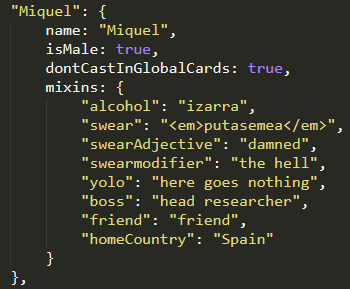
\includegraphics[width=8cm]{figures/2-Ice-Bound/casting-data.png}
    \caption{A character definition within the level definition file.}
    \label{fig:casting}
\end{figure}

%%%%%%%%%%%% END FIGURE %%%%%%%%%%%%%%%%%%%%%%%%%%%%%%%%

\paragraph{Level Definition.}\label{par:icebound-level-definition}

Level definition files are the heart of each level. They define characters, which symbols are available where, and all the art and music files. While the specifics of what values each one would have takes some time to develop, overall these were fairly lightweight to work with. The majority of their contents are actually concerned with the visual appearance and arrangement of items on-screen for the level, and therefore don't come into play as much during the content authoring stage.

We would also define here any custom ``mixins" that could be used by state templates to customize story text to fit particular characters. For example, in an event card about a confrontation with an authority figure (the ``boss" mixin in Figure \ref{fig:casting}) that might be a ``head researcher" in Miquel's case, or a ``government official" or ``naval captain" for different characters.

\paragraph{Cards (Symbols, Events, Endings)}\label{par:cards-symbols-events-endings}

What we call ``cards"---the individual units of content for the digital story in \textit{Ice-Bound}---were the main focus of authoring. The amount of overhead for writing a card was fairly low: one could start by writing a card statically-cast to a certain character, with static text, then go back in and start adding more dynamism progressively, until either the cognitive overhead was too high, or the desired complexity was met. In the case of the former, more cards could be added with conditions to help cover the possibility space between an associated group of cards.

%%%%%%%% BEGIN FIGURE %%%%%%%%%%%%%%%%%%%%%%%%%%%%%%%%%

\begin{figure}
    \centering
    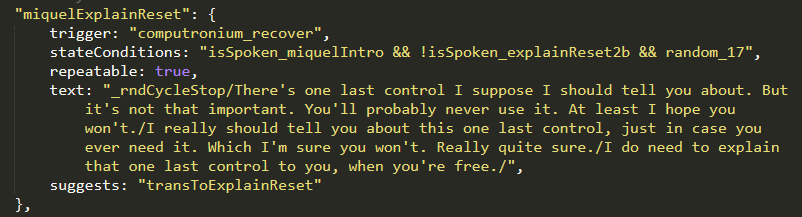
\includegraphics[width=\textwidth]{figures/2-Ice-Bound/dialogue-data.png}
    \caption{Sample JSON from an event card, with character and state templates.}
    \label{fig:dialogue-data}
\end{figure}

%%%%%%%%%%%% END FIGURE %%%%%%%%%%%%%%%%%%%%%%%%%%%%%%%%

These dynamisms could compound to become rather complex. In the example of Figure \ref{fig:dialogue-data}, we can see simple pronoun grammars, but also ones like \newline
``\_socket/miquel5/traitAdjective/." Because each symbol card comes with an associated adjective to describe the character, such as ``lucky" or ``foolhardy", this means you can reference that trait in subsequent cards, as long as we can ensure that character is cast. Because the template refers to a specific socket ``miquel5", which (perhaps somewhat confusingly) is always in Stanley's room, and Stanley is always cast as ``character a", we know by design that this will always line up.

Another interesting use of templates in this card is ``\_socket/miquel4/itemNoun/", which takes the symbol card's object, and inserts that into the text. Since the socket ``miquel4" in this case is a global symbol card, and symbols are always objects, we can get a nice spread of interesting things that Stanley keeps hidden away, and whoever is cast as character b can discover by picking the lock on their room.

While in terms of the discretely different things to be written for one piece of content is relatively low, this example shows how more complex and interesting permutations can be quite labyrinthine to craft. Often for these more complex cards, we would start with a premise (``an event where a character breaks into another's room and sees what's in there") and work from there, as opposed to writing static text, and then making it more generative afterwards.

\paragraph{KRIS Dialogues.}\label{par:kris-dialogues}

%%%%%%%% BEGIN FIGURE %%%%%%%%%%%%%%%%%%%%%%%%%%%%%%%%%

\begin{figure}
    \centering
    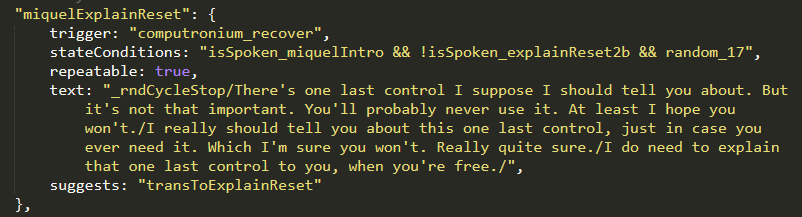
\includegraphics[width=\textwidth]{figures/2-Ice-Bound/dialogue-data.png}
    \caption{A sample KRIS dialogue.}
    \label{fig:kris-dialogue-data}
\end{figure}

%%%%%%%%%%%% END FIGURE %%%%%%%%%%%%%%%%%%%%%%%%%%%%%%%%

The branching dialogues with KRIS were similarly simple to create. Triggers and state conditions controlled when they appeared, which could come from player actions such as activating a symbol, other dialogues being triggered, or even randomly with a given percentage (shown in Figure \ref{fig:kris-dialogue-data}'s stateConditions as ``random\_17"). This text could be made more dynamic later on by going in and adding state-driven templating, or even just random variances for recurring dialogue prompts (as seen in Figure \ref{fig:kris-dialogue-data}). These dialogues could chain immediately to the following one by id, through the field ``suggests." They could also contain an ``options" array which would route the player accordingly once they picked the corresponding choice.

\paragraph{Book Pages}\label{par:book-pages}

Book pages were straightforward to create, being composed of static text or graphical elements, and then a secondary AR element. While they did have themes and tags applied to them, they were more authored as static conceptual narrative support for the digital narrative, to provide longer context and clues for what was going on when KRIS had written drafts of these stories while human. Writing this type of content required equal parts traditional narrative skills, as well as graphic design skills (for layout and design). This proved no problem for the authors, as they could leverage their common professional skillset from previous work as graphic designers.

\subsubsection{Clarity}\label{par:icebound-clarity}

Given the different layers of combinatorics between symbols, events, endings, KRIS dialogues, and theme resolution within the printed book, \textit{Ice-Bound} has complex system dynamics, although each individual piece on its own doesn't pose a particularly high degree of challenge. While it wasn't usually the case that newly authored content could modify state in such a way that necessary later cards were invalidated, the space needing content coverage was complex enough that tools were necessary in order to be sure that we had written enough content to account for all the different combinations of symbols a player may activate in the course of a playthrough. This is the area where we chose to spend most of our labor, in order to reduce the authorial burden. Without assistance here, the authoring task would have become too opaque for us to make consistent progress, and we would have no clear idea of when we had authored enough content to ensure the game was playable.

To avoid that, we essentially wanted to know two things: 

\begin{enumerate}
    \item How many combinations are needed for state coverage without an unattainable amount of writing?
    \item How can we know when we've accomplished coverage for all cases?
\end{enumerate}

In the course of development, we created three different content library visualization approaches to answer these questions. Because they are a bit involved, we'll first talk briefly about previous work in this area, in order to contextualize our decisions.

\paragraph{Historical Visualization Approaches}\label{par:historical-visualization-approaches}

Visualizing possible states the player may explore in a given piece is an authoring problem that’s been addressed in a number of different ways. The most prevalent visualization for interactive narratives is the simple graph (including trees), where nodes are individual story segments (or lexias) connected via the afforded actions of the player. Hyperfiction, for instance, typically uses the display of node connections to show the afforded action of clicking a link. These graph visualizations have been in place since the early days of non-linear storytelling with tools like Aquanet \cite{shipman1999spatial} and Storyspace \cite{bernstein_2007}, and continue to be used today in a variety of authoring tools, from Twine \cite{klimas2008twine} to game modding tools like the Neverwinter Nights toolsets \cite{nwnwiki_2019}. 

These sorts of graphs fill the most immediate need of authors: seeing the overarching structure of a piece, providing a way to see where paths of interaction dead end, where concentrations of links make certain content more likely to be displayed, or the lack of links makes it perhaps impossible.

As said by Mark Amerika, author of Grammatron: ``creating complex hypertext structures for the web is a nightmare because, after a certain point, one cannot visualize a cognitive mapping structure for a webwork that has literally thousands of screens and links" \cite{bernsteinamerika}. In this case, Storyspace’s ability to provide a simple spatial representation of reader pathways proved invaluable to his efforts. Another interesting aspect of tools such as Tinderbox \cite{tinderbox} and Twine, is that the authoring interface can be heavily bound up in the visualization itself, where creating a new node in the visualization directly maps to creating a new node in the work. Semantic flags in the writing itself can create new nodes, which are immediately added to the visualization. In these sorts of environments, the authoring is done from within the data visualization of the media artifact rather than as a response to experiencing the game or text, which (through leveraging good UI design) can dramatically increase an author’s ability to architect complex narrative structures. 

Games that provide powerful tools for the creation of new narratives with game engines, such as the Neverwinter Nights toolsets, still hold to the graph structure for narrative visualization, if they provide one at all. The well-used tree map for branching dialogue with NPCs is still the standard, and well-suited to most forms of menu-driven interaction with game characters. But it also begs the question: with different, more sophisticated visualizations, what narratives could become feasible to create?

Another visualization tool for interactive narrative debugging is the IDE for Inform 7, a parser-based interactive fiction language, which features a view of possible story traversals called the ``Skein." This mode also makes use of a graph metaphor, although with the graph now showing multiple playthroughs of the interactive narrative, which can be replayed upon changes to the narrative code to ensure they still produce the expected output. This opens up interesting diagnostic affordances to authors, allowing them to zero in on specific series of actions taken by players \cite{reed_inform}. However, this visualization has trouble addressing IF’s sheer combinatorial scale. The basic player affordance to interact via an arbitrary combination of nouns and verbs (``get lamp", ``drop lamp", ``light lamp") quickly becomes too large to be tenable for visualization, and would even perhaps not be considered useful. In general, it isn’t sensible to author dedicated content for nonsensical parser commands, such as ``eat lamp." Therefore, the easiest way to generate data for visualization falls back to playtraces, which can rely generally on players to engage in goal-directed play that avoids nonsensical parser command combinations.

Continuing in this vein, research into aggregating playthrough data into playtraces (such as Liu et al's work \cite{playtraces}) provides representations that could be adapted to provide narrative diagnostic strategies for projects where readers have a high level of expressive affordance. For example, Osborn's \textit{Gamalyzer} \cite{Osborn_playtracer} generates graph structures where certain nodes are defined as goal states, and each choice or state the player can induce in the system is a node connected by the action to the previous state. This emphasis on player actions as opposed to game states is well-suited for adaptation to narrative concerns, where many times the focus is on the variety of available player actions or affordance.

There have also been playthrough visualizations used for interactive narratives to better understand the potential space explored through interaction. For \textit{Prom Week}, a game making use of cutting-edge persistent social state modeling to create dynamic experiences for each player, visualization served a critical evaluative purpose in exposing how quickly individual playthroughs become unique \cite{promweek_playtraces}. These same techniques were used to demonstrate a similar property in \textit{Façade}, an earlier work famous for its expressive player affordances.

\paragraph{Design Goals}\label{par:icebound-design-goals}

The goal of the visualization system was to highlight where symbol combinations did not trigger at least three events and two endings, our self-selected minimum requirement for content. Symbol combinations where this is not the case needed more authoring. This metric was also parameterized, such that we could make it stricter later on in the authoring process, to provide finer feedback. When considering where new content would be most useful, the primary consideration was discovering a combination of symbols to be used as a precondition that filled existing holes in the possibility space. The visualization needed to provide information to allow authors to intuitively grasp how to accomplish that. \textit{Ice-Bound}’s engine is written in Javascript, so the visualization tool also needed to run on the same code base. This was necessary to minimize errors that might be introduced through re-implementation of game procedures, and also to ensure any future changes introduced to those game procedures would be faithfully reflected in the visualization. Ideally, the tool would both provide a window on the possibilities for an example level build (where all the symbols have been selected for sockets) and reveal possible level builds where there were not enough events or endings written or triggered, if certain symbols were involved. Furthermore, showing us which specific symbol combinations give rise to these states would give strong indicators for authoring appropriate preconditions to new events and endings in order to fulfill our goals.

\paragraph{System Description}\label{par:icebound-system-description}

The system was designed in two parts: a combination browser and a level profiler. The browser is concerned with broadly classifying combinations which need content, abstracted from a specific level build. The profiler gives a detailed view into the combinations within a specific level build. In operation, the combination browser is used to provide a list of explicit symbol combinations where content is sparse. The user can then click those combinations to build a level containing the given symbols, and through the level profiler, see how much content is needed to fix the scarcity issue.

\paragraph{Combination Browser}\label{par:icebound-combination-browser}

The combination browser engages all possible symbol activations for a level by permuting every unique combination of symbols from the global pool and level-specific pool of symbol cards, equal in length to the amount of available ``lights" on the level (the objects players manipulate to activate symbols) as specified in the levelDef file. It then uses the game logic to simulate activating each symbol, rebuilding the level if necessary to contain those symbols. If the level cannot be built with a particular combination of symbols (i.e. a symbol has a precondition precluding it being chosen if another symbol is present) it discards the combination as illegal. After each activation of symbols on this simulated level, the system records the number of events and endings activated.

Once the system has permutated through all valid symbol activation combinations and constructed this exhaustive list of events and endings, it decomposes the combinations such that it has a record of how many under-authored combinations each symbol is part of. For example, if the symbol combinations A, B, C and A, C, F both lack the appropriate number of events and endings, the system would yield that both A and C are part of two problematic combos, while B and F are only part of one.

This analytical strategy was chosen because the most direct solution to the problems highlighted by the viz is authoring more event and ending cards, with preconditions containing the specific symbols suggested. Thus, a symbol's presence in more than one combination inadequately covered by content is a good candidate for a precondition in future content.

Again, our goal is to increase system dynamics clarity for authors. Therefore, an important quality of this visualization is that it happens quickly enough to make it useful for making small changes and seeing how that affects the possibility space. Furthermore, once formulated, the data in the visualization can be quickly manipulated, which greatly increases its utility.

%%%%%%%% BEGIN FIGURE %%%%%%%%%%%%%%%%%%%%%%%%%%%%%%%%%

\begin{figure}
    \centering
    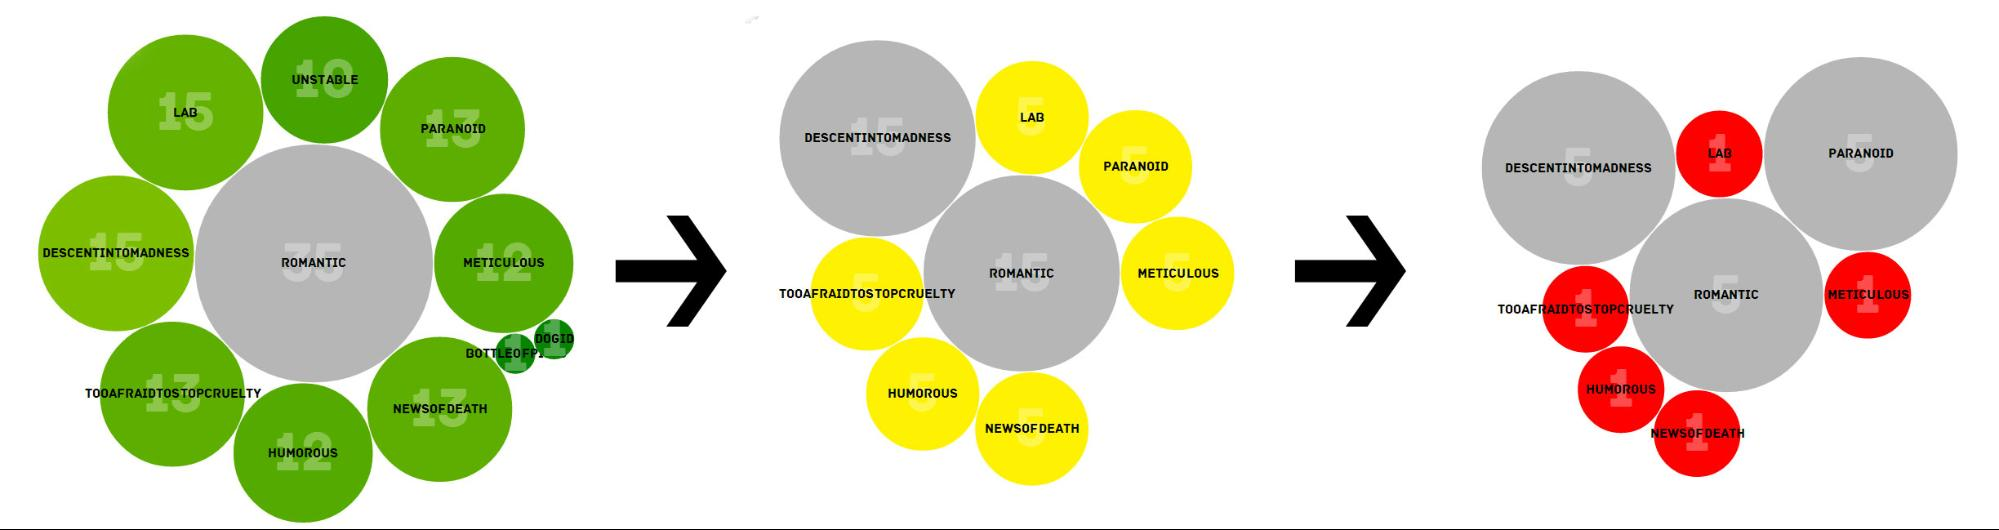
\includegraphics[width=\textwidth]{figures/2-Ice-Bound/bubble-viz.jpg}
    \caption{The combination browser, as the viewer progressively zeros in on problem combinations by clicking the symbol ``romantic", then ``descentIntoMadness", then ``paranoid."}
    \label{fig:bubble-viz}
\end{figure}

%%%%%%%%%%%% END FIGURE %%%%%%%%%%%%%%%%%%%%%%%%%%%%%%%%

\paragraph{Display Strategy}\label{par:icebound-display-strategy}

The browser displays each symbol as a circle in a bubble cluster diagram (Figure \ref{fig:bubble-viz}). The size of the bubble corresponds to the number of problematic combinations the symbol was involved in. Each bubble can be clicked to tell the system to apply the same visualization methods on the subset of combinations involving only the selected symbol. Doing this resizes the other bubbles in the visualization, so their new size corresponds to the number of times they are involved in a problematic combination with the new set of selected symbols. If a different bubble is clicked, the values are again updated. This allows the viewer to interactively evaluate and discover problematic symbol combinations.

There is a specific tension in authoring goals when trying to patch content holes. On one hand, the more combinations an authored event or ending hits, the more effective it is at patching a hole. However, if its pre-conditions mean it is also being activated for combinations which do not need more events and endings, it is potentially diluting that space. During gameplay, if a combination triggers more than five events or three endings, we truncate the list in order to keep the scope of the stories presented to the player from becoming overwhelming. However, the ranking policy we use to determine which to cut is very simplistic; additionally, there's always the risk that the ones we cut have an implicit connection to the symbols that is reflected in the authored surface text, but not reflected in nuanced ways in the content tags. If such events or endings are cut, it's possible it could lessen the perceived causal link between the player's choices and the system's response. Therefore, the closer we can keep all combinations to five events and three endings, the less we need to cut, and the higher the perceived causal link for the player from their actions to the reaction of the system.

To reflect these tensions, a ``traffic light" circle color scale from green to red was adopted to show the ratio of combinations needing content versus not needing content. Red circles have the highest ratio of content-less combinations, and green circles have the least. This is necessary in order to discourage the authoring of content with pre-conditions that trigger for combinations that don't need it. For example, while authoring an event with pre-conditions that trigger for every combination in the game would technically address every combination needing content, it would also appear for many combinations that didn't need additional events and endings. Also, from a narrative design standpoint, the more targeted an event or ending is to its precondition symbols, the better. It leads to content that strongly correlates with the player's selection, communicating that their choices are having a real effect, and that they have agency over the story being formed. Events or endings that show up for many different combinations are also more likely to conflict in some way with other content that is selected.

This means that the author can quickly browse to symbol groups that both have a high content need in their combination sets (by selecting circles with redder color) as well as representing a large number of the total combinations needing content for the level (by selecting circles which are larger).

Because the specifics of this are difficult to grasp, there is an additional info panel that displays the same information as the color and size, using text and tooltips (Figure \ref{fig:viz-detail}). The color, which is determined by the ratio of combos needing content, is reflected as a pie chart (C) with explicit text (B). The size of the circle is also shown numerically (D).

%%%%%%%% BEGIN FIGURE %%%%%%%%%%%%%%%%%%%%%%%%%%%%%%%%%

\begin{figure}
    \centering
    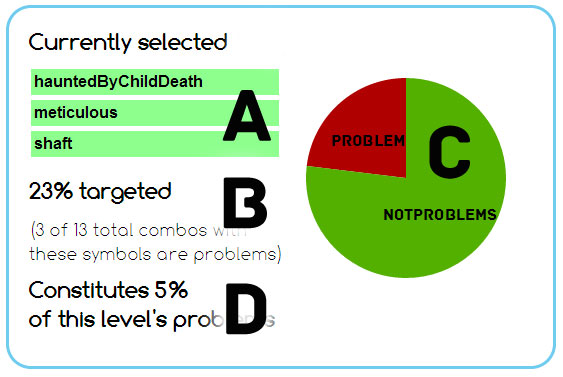
\includegraphics[width=\textwidth]{figures/2-Ice-Bound/viz-detail.jpg}
    \caption{The detail panel in the combination browser, showing the selected symbols (A), and the percentage of their combinations which need content (B), also represented by the pie chart (C). (D) shows how many of the total combinations needing content the current selection is involved in.}
    \label{fig:viz-detail}
\end{figure}

%%%%%%%%%%%% END FIGURE %%%%%%%%%%%%%%%%%%%%%%%%%%%%%%%%

While providing a good top-down view of the content distribution as a whole, the combination browser does not show the content distribution within run-time combinations of a particular level build. This gives rise to a blind spot in authoring considerations. If the combinations lacking content are concentrated in a few specific builds of a given level, that is a bigger problem than a low number of problems that persist across all possible level builds. For example, if only 1 out of 35 content-lacking symbol combinations is present in a level build, it isn't as glaring a problem as all 35 problems being present in one level build, due to the fact that a given level build can have around 30-70 combinations. In the first case, only 1.4 - 3\% of the player's possible chosen combinations are lacking. In the second case, it's closer to 50 - 100\%.

To address that, we needed a visualization dealing with specific level builds, accessible via the combination browser. This is accomplished through listing out the symbols currently being inspected by the viewer. If the symbols ``romantic", ``descentIntoMadness", and ``paranoid" are selected, the list contains every content-needing combination containing those symbols, with a link to ``build." When clicked, the system builds the level containing those symbols, and displays the second visualization tool: the level profiler.

\paragraph{Level Profiler}\label{par:level-profiler}

The level profiler (Figure \ref{fig:bar-viz}) was the visualization most used during the initial round of authoring for \textit{Ice-Bound}. It displays the run-time combinations of a given level build with a given set of symbols in the form of an annotated stacked bar graph. Each bar represents a particular set of active symbols, with the height corresponding to the total number of events and endings it activates.

%%%%%%%% BEGIN FIGURE %%%%%%%%%%%%%%%%%%%%%%%%%%%%%%%%%

\begin{figure}
    \centering
    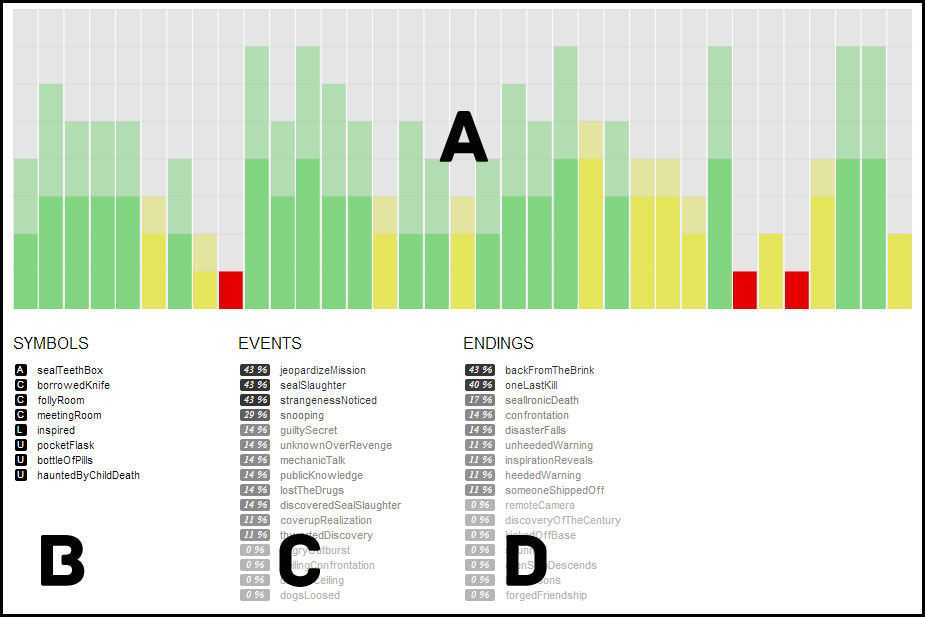
\includegraphics[width=\textwidth]{figures/2-Ice-Bound/bar-viz.jpg}
    \caption{The level profiler for \textit{Ice-Bound}, showing all possible run-time combinations of active symbols for a single build of a level. Red bars indicate content-sparse combinations. Clicking on specific Symbols (B) Events (C) or Endings (D) will re-sort the graph (A) to lump combinations using those cards together.}
    \label{fig:bar-viz}
\end{figure}

%%%%%%%%%%%% END FIGURE %%%%%%%%%%%%%%%%%%%%%%%%%%%%%%%%

The bottom portion of the bars represents events, and the upper portion endings. This provides an easy way to see which combinations do not trigger enough content. The coloration of these bars is either green, yellow, or red. This is dependent again on the two combination minimums we established for a ``satisfying" story: a combination should trigger at least three events and two endings. If a combination satisfies both of those, it is green. If it only satisfies one, it is yellow. If it satisfies neither, it is red.

Below the graph are a list of the symbols present in the level, as well as every event and ending that can be logically triggered by those symbols. Hovering over a given bar in the chart highlights the symbols, events, and endings activated in the lists below. Additionally, each item on the lists below the chart can force a re-sort of the chart upon being clicked. This means if authors want to see content authored for a specific symbol, event, or ending, they click on it, and the graph re-sorts so that all combinations involving that move to the left.

This proved enormously useful in highlighting problems that weren't readily apparent from the complex interactions of pre-conditions for various events and endings. Red bars indicating problem sets of active symbols could be examined to look for common elements, indicating there were not enough events and endings activated by those elements. Using this tool, one could quickly see what the combinations that need more content have in common, and get a feel for how much content is currently available to the reader at run-time. In this way, clarity for authoring was greatly increased.

\paragraph{Pragmatic Tables}\label{par:pragmatic-tables}

In addition to these data visualizations, which took a significant amount of time to build out, test, and deploy, we also used a ``quick and dirty" method to audit combinations. This took the form of a webpage that displayed several tables.

%%%%%%%% BEGIN FIGURE %%%%%%%%%%%%%%%%%%%%%%%%%%%%%%%%%

\begin{figure}
    \centering
    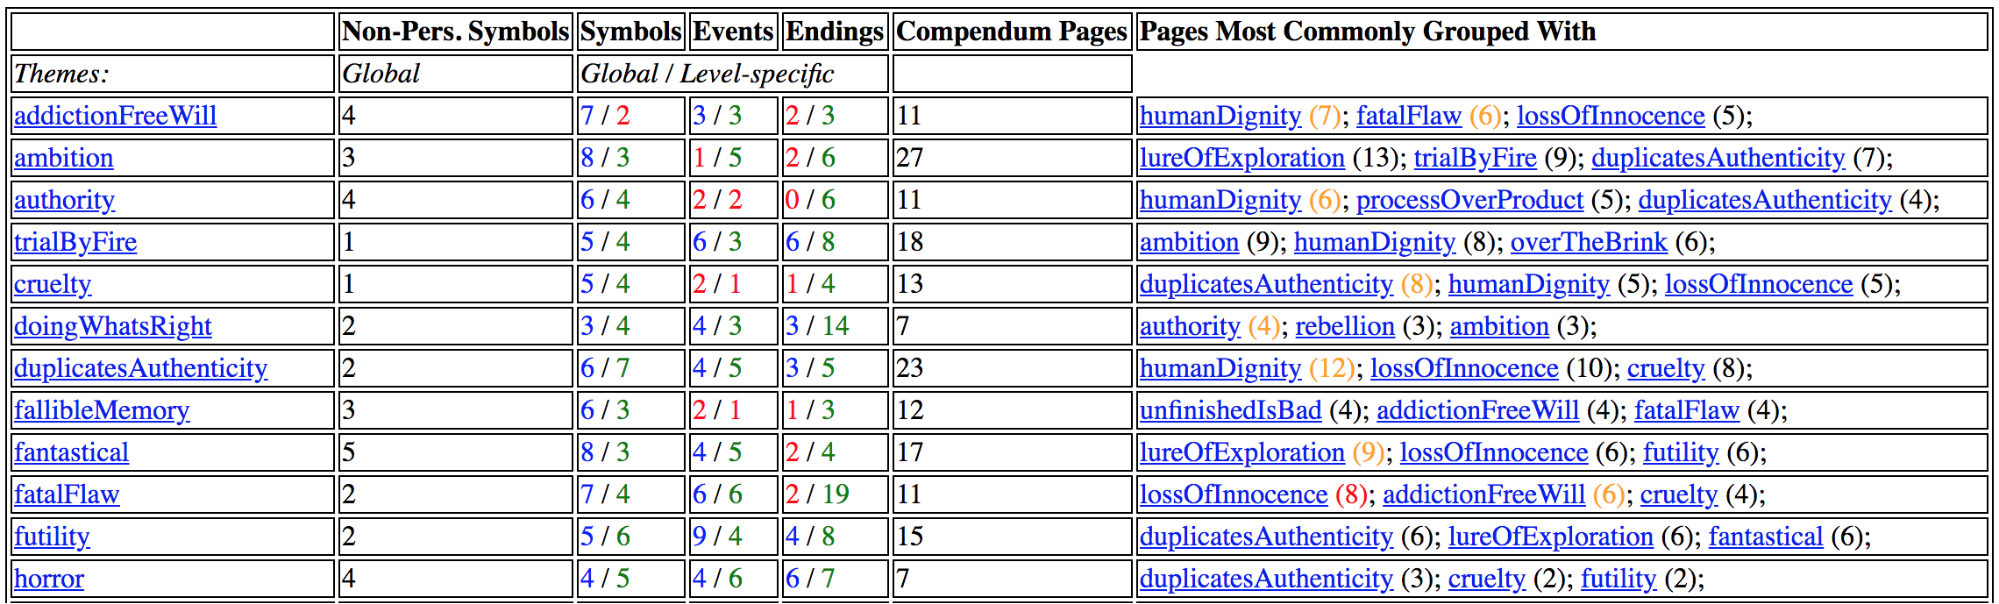
\includegraphics[width=\textwidth]{figures/2-Ice-Bound/pragmatic-tables.png}
    \caption{A table selection showing themes, as well as how many symbols, events, and endings use it.}
    \label{fig:prag-tables}
\end{figure}

%%%%%%%%%%%% END FIGURE %%%%%%%%%%%%%%%%%%%%%%%%%%%%%%%%


As seen in Figure \ref{fig:prag-tables}, each theme is listed, along with how many global or level-specific cards implement that theme for the three types of content cards. Numbers are color-coded red when there is less than a viable amount written. This makes it simple to see at a glance which themes are most in dire need of content.

This same page also has a simple text listing of ``pages with fewest themes", ``tags/themes most used as preconditions", ``tags/themes least used as preconditions", ``cards most used as preconditions", and ``cards least used as preconditions", arranged from highest value to lowest value. This provided us a barebones way to avoid over-using themes, which as mentioned in discussion of the more elaborate visualization, dilutes their perceived effectiveness to the reader.

%%%%%%%% BEGIN FIGURE %%%%%%%%%%%%%%%%%%%%%%%%%%%%%%%%%

\begin{figure}
    \centering
    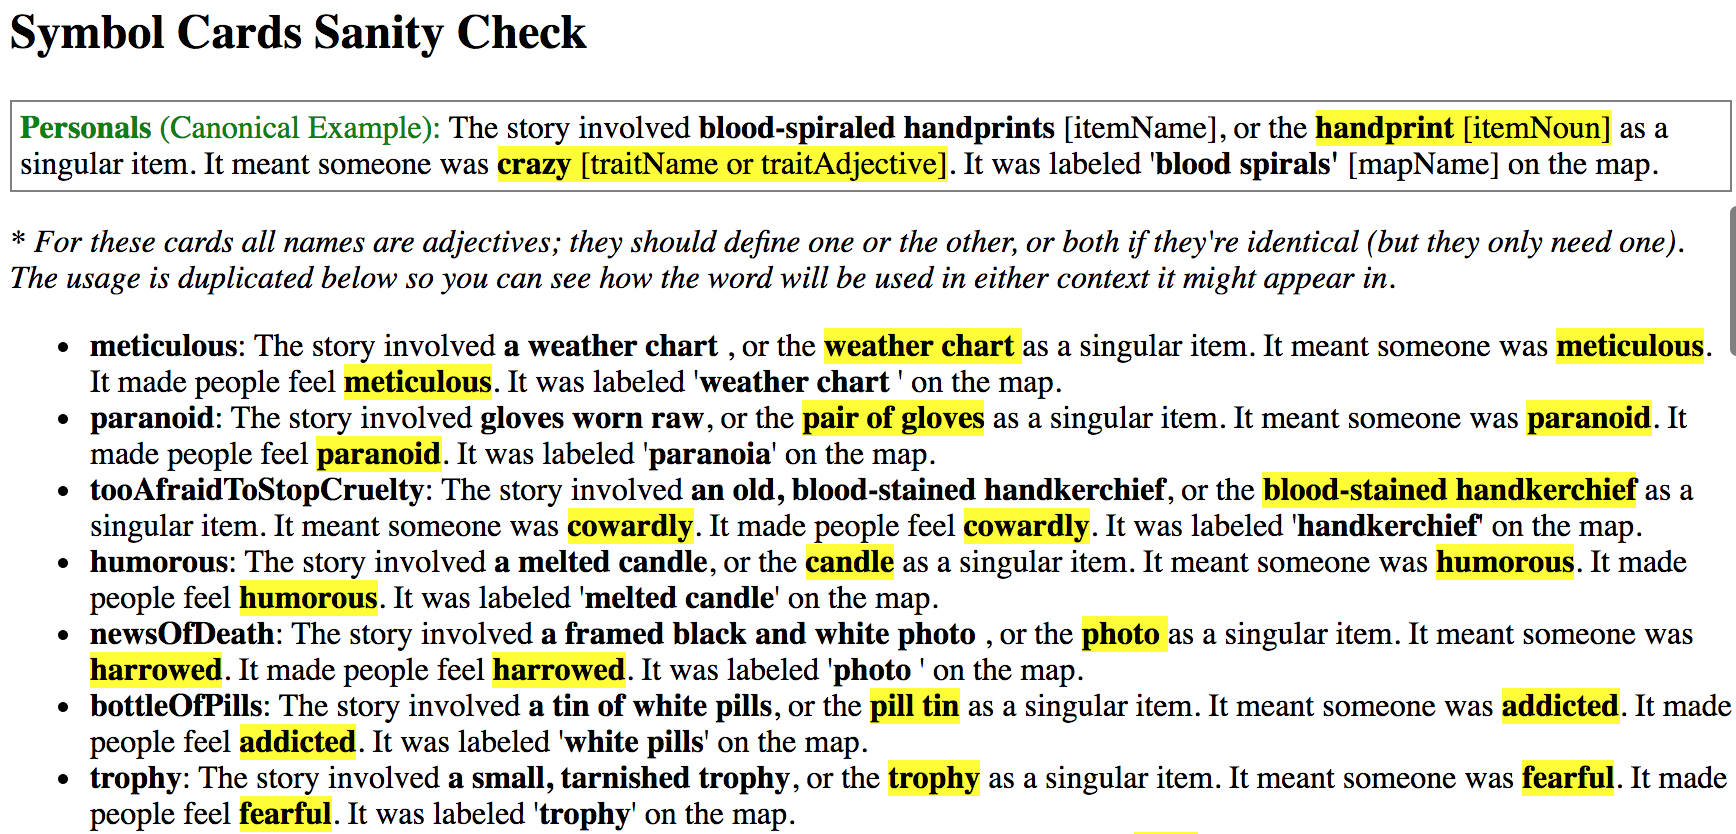
\includegraphics[width=\textwidth]{figures/2-Ice-Bound/symbol-checker.png}
    \caption{Rendered text for symbols, to check for coherence.}
    \label{fig:symbol-checker}
\end{figure}

%%%%%%%%%%%% END FIGURE %%%%%%%%%%%%%%%%%%%%%%%%%%%%%%%%

A separate section displayed all the ways a symbol card could be used in a sentence. This let us audit the creation of new content that might be combined in surprising ways, to ensure it would remain grammatically correct regardless of where it appeared.

\subsubsection{Controllability}\label{subsubsec:icebound-controllability}

The Controllability requirement for \textit{Ice-Bound} was, taking all things into consideration, roughly Medium. Despite the firm target of at least three events and two endings for every combination in the level, we were helped by the aesthetic decision to keep story segments relatively self-contained (which is reflected in the Medium level of Contextuality). This meant that surprising juxtapositions could be plausible explained by the reader as long as the leaps weren't too far, keeping in mind the design mantra of Failbetter's ``fires in the desert." The level profiler and combination browser visualizations here also allowed us to quickly browse through existing combinations, to find situations where badly written preconditions resulted in strangely triggered (or mis-triggered) events and endings. All in all, most events and endings in \textit{Ice-Bound} are adequately controlled by pre-conditions with just three to five terms, all of which are simple booleans checking for the activation of other cards or certain tags.

In terms of the surface text (and in order to support surprising juxtapositions by providing some supporting consistent details) we did want to exert strict control over the casting of characters. This was both to ensure their role persistence through the stories aggregated from the triggered cards, as well as their dominant qualities, since the stories were, aesthetically speaking, predominantly character studies. This we accomplished with the aforementioned DSLs and state-driven templating. However, we also were able to reduce authorial burden here by framing some tricky templating instances as shimmer-text, which allowed us to both showcase the potential variant space while providing a piquant user interaction, while also freeing ourselves from the need to track more variables to do it automatically. This quality parsimony, to borrow another term from Failbetter, also helped keep things relatively simple and increase authorial Clarity as we created content.

\subsubsection{Authorability Summary}\label{subsubsec:icebound-authorability-summary}

Of the three main projects discussed in this dissertation, \textit{Ice-Bound}'s authoring tools were the most well-developed by far. Relatedly, \textit{Ice-Bound}'s content creation system was also the one most ``put through its paces" to create a shippable narrative experience, both in terms of volume and quality.

Because the state and system dynamics of the experience were complex, these different approaches and strategies each provided a lens we could use as authors to increase Clarity, by simplifying those dynamics to either an integer in a list, or a simple visual representation of circles and colors. Also, negative feedback was prominent enough that when content was made that had bad dynamics, it was immediately obvious.

These tools were run continuously throughout content creation for the process, and could give feedback immediately. Because of this, it was easy to create a "todo list" of cards for a given writing session, with specific constraints which---while at a given point the writer may not know how it fits into the bigger picture---mean they will be increasing our content pool as efficiently as possible. The distillation of this was our one sentence prompt at the top of the tables page, which might read something like ``Why don't you write an event or ending card about theme\_ambition (5) triggered by tag\_mazeMemory (1)?"

Towards the end of the writing process, the increasingly-specific constraints took on a form of writing under constraint (reminiscent of the aforementioned Calvino work \textit{Mr. Palomar}) which was actually more of a pleasant challenge than an onerous or confusing burden. Even if the writer came to the table with a certain event or character development they wanted to use, they could then say ``how can I change this such that it's also about ambition, or rebellion." And if a given thematic combination was too difficult to author, these visualizations allowed us to easily find alternate ways to satisfy the requirements using different thematic combinations, despite the complex dynamics at play.

Thus, despite the Complexity being fairly high for authoring content, it was ameliorated by the Clarity afforded by our feedback solutions. Because of aesthetic decisions that meant each card was relatively self-contained, and the aforementioned visualization tools, we could get away with a roughly medium amount of Controllability. And because the Proficiency required for authoring was evenly matched with the author's skills (easily achieved, since we were the only authors!) the net result was a design and creation process with high authorial leverage.

\section{System Summary}\label{sec:icebound-system-summary}

\textit{Ice-Bound} was a successful project, from conception to finished media experience, because we managed to thread the needle of runaway combinatorial authorial burden with solutions to curtail it, and make the content needed for our systems pull double-duty. Our initial concept of the project was one that would require high Traversability. Because of the time invested in paper prototyping and iterating on simple digital prototypes, we were able to zero in on the key ways we wanted the system to shine: high Explorability (through the ``sculptural fiction" mode of interaction) and Replayability, through the use of high Contextuality. In order to help meet that challenge, we put in place designs from the beginning that would help reduce the amount of authoring needed by increasing content Reusability, through card availability in multiple contexts, and cards fulfilling multiple spots in the content library for different sets of preconditions, assisted by the state-driven templating.

In order to meet this content creation challenge, we needed to increase our Authorability as much as possible. Because the content authors were also the system engineers, we were able to get away with a relatively high requirement for Proficiency, while still having the friction for authoring remain fairly low. The many different components required for authoring (cards, KRIS dialogues, Compendium pages) pushed the Complexity high.

However, because of the amount of effort spent on tools---from the simple-yet-informative ``pragmatic tables" to the more exhaustive combination browser and visualizer---we were able to increase our Clarity greatly. These tools enabled us to zero in quickly on bad dynamics or holes in our content library, and also determine when we needed to find ways to increase the reusability of particular pieces of content, and when we needed to simply roll up our sleeves and get to work.

\section{Next}\label{sec:icebound-next}

\textit{Ice-Bound} was a successful endeavor, from both a research and media production standpoint. However, many things were already working in its favor. And while it was still an experimental work by many metrics, many of the decisions made in its development ``reigned it back" in service to releasing a finished product to a waiting audience. Features were cut early on, capabilities that could have pushed the procedurality further were left for ``the sequel" (a facetious phrase we used to make the parting easier) ensuring we could finish a polished work using the system.

Next, we turn to the familiar domain of choice-driven narratives. Driven this time more by a research mandate for the creation of a novel system with a wide array of experimental narrative affordance, we were able to push the boundaries a bit further. The result was a system that advances the evolution of dynamically-assembled choice-based narrative, but fought against ever-escalating authorial complexity. In the course of that fight valuable insights were gained, both in system architecture and narrative design, and resulted in both a publicly available narrative engine, and a finished research game: \textit{Emma's Journey}.

